\documentclass[12pt,a4paper,final,twoside]{article}
\usepackage[utf8]{inputenc}
\usepackage[catalan]{babel}
\usepackage{url}
\usepackage{graphicx}
\usepackage{hyperref}
\usepackage{amsmath,amssymb,amsthm,amscd}
\usepackage{setspace}
\onehalfspacing
\usepackage{multirow}
\usepackage{caption}
\usepackage{subcaption}
\usepackage{framed}

\usepackage[ampersand]{easylist} 
\usepackage{epstopdf}
\usepackage{array}
\usepackage{tabulary}

\usepackage{float}

\usepackage[left=2.5cm,right=2.5cm,top=2.5cm,bottom=2.5cm]{geometry}

\usepackage{appendix}
\renewcommand{\appendixname}{Annexos}
\renewcommand{\appendixtocname}{Annexos}
\renewcommand{\appendixpagename}{Annexos}
\makeindex

\usepackage{wrapfig}

\usepackage{fancyhdr}
\pagestyle{fancy}
\fancyhead{}
\fancyhead[RO,LE]{\thepage}
\fancyhead[RE,LO]{Sincronització amb aibo}
\fancyfoot{}
\fancyfoot[RO,LE]{
\includegraphics[scale=0.3]{images/etseib.jpg}}

\headheight = 15pt 

\textheight = 690pt 
\footskip = 60pt

\usepackage[numbers]{natbib}
\usepackage{listings}
\usepackage{color}

\definecolor{mygreen}{rgb}{0,0.6,0}
\definecolor{mygray}{rgb}{0.5,0.5,0.5}
\definecolor{mymauve}{rgb}{0.58,0,0.82}

\lstset{ %
  backgroundcolor=\color{white},   % choose the background color; you must add \usepackage{color} or \usepackage{xcolor}
  basicstyle=\footnotesize,        % the size of the fonts that are used for the code
  breakatwhitespace=false,         % sets if automatic breaks should only happen at whitespace
  breaklines=true,                 % sets automatic line breaking
  captionpos=b,                    % sets the caption-position to bottom
  commentstyle=\color{mygreen},    % comment style
  deletekeywords={...},            % if you want to delete keywords from the given language
  escapeinside={\%*}{*)},          % if you want to add LaTeX within your code
  extendedchars=true,              % lets you use non-ASCII characters; for 8-bits encodings only, does not work with UTF-8
  frame=single,                    % adds a frame around the code
  keepspaces=true,                 % keeps spaces in text, useful for keeping indentation of code (possibly needs columns=flexible)
  keywordstyle=\color{blue},       % keyword style
  language=Octave,                 % the language of the code
  morekeywords={*,...},            % if you want to add more keywords to the set
  numbers=left,                    % where to put the line-numbers; possible values are (none, left, right)
  numbersep=5pt,                   % how far the line-numbers are from the code
  numberstyle=\tiny\color{mygray}, % the style that is used for the line-numbers
  rulecolor=\color{black},         % if not set, the frame-color may be changed on line-breaks within not-black text (e.g. comments (green here))
  showspaces=false,                % show spaces everywhere adding particular underscores; it overrides 'showstringspaces'
  showstringspaces=false,          % underline spaces within strings only
  showtabs=false,                  % show tabs within strings adding particular underscores
  stepnumber=2,                    % the step between two line-numbers. If it's 1, each line will be numbered
  stringstyle=\color{mymauve},     % string literal style
  tabsize=2,                       % sets default tabsize to 2 spaces
  title=\lstname                   % show the filename of files included with \lstinputlisting; also try caption instead of title
}
\bibliographystyle{plainnat} 
\title{Sincronització amb AIBO}
\author{Diego Muñoz Galan}

\begin{document}

\maketitle
\thispagestyle{empty}

\newpage
\paragraph{}
\thispagestyle{empty}
\cleardoublepage

\setcounter{page}{1}

\begin{abstract}
\addcontentsline{toc}{section}{Resum}

\end{abstract}

\newpage
\cleardoublepage

\tableofcontents
\newpage
\listoffigures
\newpage
\listoftables
\newpage


\section{Prefaci}
\subsection{Motivació}
Fa ja 8 anys que l'empresa Sony va deixar de produir la mascota robòtica per excel·lència, el gos AIBO. Des de la seva desaparició del mercat ha caigut en una espiral de desús fins que avui en dia gran part d'ells estan agafant pols al fons d'un armari.

Aquest projecte va partir de una idea de tornar aprofitar els AIBOS per realitzar tasques de cooperació entre ells partint de la part alta de la programació. En vista de la incomoditat per tal de programar la plataforma en qüestió degut a dos factors el primer: l'us de llenguatges i de APIs poc usades en el mon de la robòtica i que tenen corbes de aprenentatge molt costoses a l'inici. El segon és el mal manteniment d'aquests llenguatges en els últims anys.
Això va portar a voler recuperar els AIBO d'una forma nova amb un del sistemes operatius actualment més usats en la robòtica, ROS\footnote{\textit{Robotics Operational System}\ref{ros}}. 

La integració de l'AIBO amb ROS facilitarà enormement la programació donant la possibilitat d'usar el gran ventall de paquets existents per aquest sistema operatiu. Per altra banda incrementara les seves capacitats de processament en front a altres mètodes donat que es controlara remotament, exprimint així les capacitats del hardware.
El fet de participar en un projecte que permeti al món de la robòtica educativa recuperar una plataforma tan emblemàtica com l'AIBO és un incentiu suficient per a la realització d'aquest. A més a més el propi aprenentatge intrínsec al projecte com és la oportunitat de conèixer ROS des de baix nivell i implementar els propis paquets necessaris és quelcom útil per a un estudiant apassionat per la robòtica. 

 

\subsection{Requeriments previs}
\section{Introducció}
En aquest apartat es definirà tant el punt de partida del projecte, el punt final on es pretén arribar com el camí recorregut i metodologia emprada. 
\subsection{Estat de l'art}
\label{estatdelart}
Es tractarà de descriure breument la situació actual de la robòtica i el compromis que requereix aquesta entre hardware i software.
\subsubsection{Robòtica}
Des de la primera definició de robot o des de la idea de robot que va exportar Isaac Asimov ha passat més de mig segle i tot i així es pot dir que la robòtica encara es troba en el seu bressol. De fet és difícil definir quin és l'origen de la robòtica i quin va ser el primer robot, el que està clar és que aquesta branca de la ciència va fer grans avanços arrel de la revolució industrial de la ma de d'altres tecnologies com l'electrònica, la informàtica o la intel·ligència artificial.

En un primer moment els robots van ser maquines automatitzades per tal de realitzar tasques que tinguessin un cert risc, requerissin de més  o eficiència que la ma d'obra humana pogués oferir dins de la industria. En aquest àmbit actualment es poden trobar braços manipuladors en la majoria de fabriques i és un fet que aquests incrementen el grau d'automatització de l'industria i amb aquest la seva eficiència\cite{libroblanco}. Un exemple d'aquest robots són els robots KUKA\footnote{\url{http://www.kuka-robotics.com/en/}} com el de la Figura\ref{fig:kuka}.
 
\begin{figure}[h!]
	\centering
    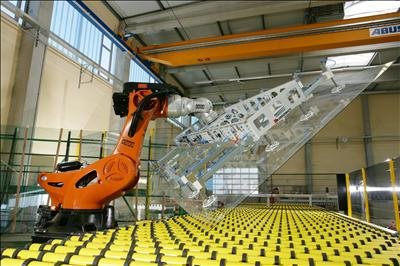
\includegraphics[scale=3]	{images/kuka.jpg}
	 \caption{Robot manipulador de KUKA.}
  \label{fig:kuka}
\end{figure}

Altres sectors apart de la industria han donat un gran impuls a la robòtica i han donat peu a la necessitat de robots mòbils. Aquest és el cas de l'exploració espacial que va tenir els seus primers passos amb el automòbil soviètic tele-operat lunokjod\footnote{\url{http://en.wikipedia.org/wiki/Lunokhod_1}} i que ara mateix té el seu màxim exponent amb el robot Curiosity\footnote{\url{http://www.nasa.gov/mission_pages/msl/}} enviat a mart en la ultima missió de la NASA. Aquests robots tenen la senzillesa de que es mouen mitjançant rodes, tanmateix existeixen robots que utilitzen extremitats per moure's. Tot i dificultar el control de l'estabilitat i complicar la dinàmica del sistema aquests ofereixen la possibilitat de caminar per una gran varietat de terrenys; un exemple és el robot quadrúpede de DARPA\footnote{\url{http://www.darpa.mil}} i Boston Dynamics\footnote{\url{http://www.bostondynamics.com/}} Wildcat mostrat a la Figura\ref{fig:wildcat}, l'altra avantatge és l'acceptació social que comporta un robot amb una morfologia familiar per a l'humà. 

\begin{figure}[h!]
	\centering
    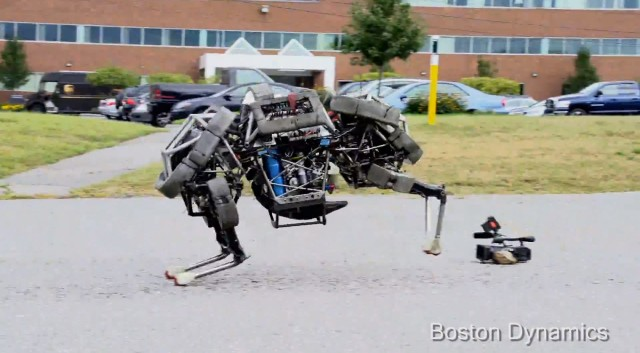
\includegraphics[scale=0.6]	{images/Wildcat.jpg}
	 \caption{Robot quadrúpede WildCat.}
  \label{fig:wildcat}
\end{figure}

\subsubsection{Robòtica en l'educació}
Aquesta ultima característica porta a la relació entre humans i robots donant lloc a robots antropomòrfics com el robot de de HONDA ASIMO\footnote{\url{http://asimo.honda.com/}} o robots mascota com és el cas de la plataforma d'estudi d'aquest projecte, l'AIBO de SONY.

Son plataformes com la que s'ha usat en aquest projecte que han permès a universitats i al públic en general interessat en la robòtica investigar a tots els nivells. Altres plataformes que han apropat la robòtica a un public molt ample permetén tant l'investigació com facilitan eines per a l'educació son els descrites a continuació:

\begin{itemize}
\item WIFIBOT: Es tracta d'una serie de robots moguts per quatre rodes amb punt d'accés wifi i que permet ser controlat i programat en varis sistemes operatius i llenguatges\footnote{\url{http://www.wifibot.com/}}.
\item Lego NXT: És un producte modular que permèt una infinitat de combinacions constructives partint sempre d'un modul de processador. Té el seu propi marc de treball\footnote{\url{http://www.lego.com/en-us/mindstorms/?domainredir=mindstorms.lego.com}}.
\item NAO: És un robot humanoide de dimensions reduïdes amb prestacions d'alta gama comercialitzat per Aldebaran Robotics \footnote{\url{http://www.aldebaran.com/en}}.
\item ARDrone:
\item DARwin:


\end{itemize}

Havent parlat d'algunes de les plataformes mes usades cal comentar, degut al compromís entre hardware i software que exigeix la robòtica, els sistemes més usats per crear la intel·ligència artificial.

La majoria de robots tenen el seu propi marc de treball que permet que aquests siguin programat en alt nivell permetent d'aquesta manera tant accedir de forma senzilla a sensors, actuadors i sistemes de comunicacions com treballar amb mòduls de programació ja elaborats amb funcions que faciliten la navegació,les comunicacions o la visió.
Tanmateix existeixen serts softwares lliures que s'estan establint com a alternativa als propis de cada plataforma. això facilita enormement la feina del programador ja que no ha d'invertir temps en prepararse per als respectius softwares de cada plataforma amb la que treballi.
D'aquests plataformes es poden destacar 2:
\begin{itemize}
\item Urbi: del qual es pot trobar informació a la secció \ref{urbi} o al annex \ref{urbiA}.
\item ROS: És el sistema operatiu de software lliure més estès actualment. Està en continu desenvolupament i abasta una gran quantitat de plataformes. Consultar la secció \ref{ros} per més informació.
\end{itemize} 

\subsubsection{L'AIBO}

Amb la plataforma AIBO secció\ref{secaibo} s'han realitzat molts projectes d'investigació degut a la seva versabilitat. Sobre tot s'han realitzat projectes relacionats amb visió\cite{xavi} o comportaments i intel·ligència artificial\cite{riki}.
Un punt essencial en el desenvolupament de l'AIBO va ser, en part,que durant el periode comprès entre 1999 i 2008 va ser el robot escollit per a realitzar la competició RoboCup Estandard Plataform League, posteriorment sustituit per la plataforma NAO. La RoboCup una competició internacional destinada a promoure la robòtica i on es realitzen probes com la esmentada anteriorment que forma part de la secció de futbol amb robots autònoms, tanmateix hi han altres probes com la competició de simulacres de rescat on l'AiBO també va ser molt utilitzat\cite{robocup}.
En aquest context de la Robocup va ser una gran motivació per a molts projectes que es poden classificar en 3 grans grups segons la finalitat: Visió i reconeixement de les marques per a la posterior situació del subjecte dins del camp\cite{morales}, comunicacions i control sobre els moviments\cite{jesus} i rols que ocupa el ròbot dins del camp\cite{metod}.

Actualment l'AIBO ja no s'utilitza com es feia avans en part per que ja no és la plataforma estandard de la RoboCup i en part perque va deixar de produir-se al 2006 per SONY i el seu llenguatge base R-CODE va deixar de ser mantingut.
A mesura que l'AIBO a quedat en desús els softwares han deixat de tenir-lo en conte, és el cas de Urbi Secció\ref{urbi} que apartir de la versió 1.5 la llibreria liburbi no és compatible amb l'Aibo. 
A més a més la recerca d'aquest projecte i sobretot la manipulació i aprenentatge dels propis llenguatges s'ha vist dificultada per la desaparició de la xarxa de gran part de la seva documentació.

\subsection{Objectius del projecte}
L'objectiu d'aquest projecte és recuperar l'AIBO com a plataforma educativa aportant-li una capa superior de programació que permeti la integració de la plataforma amb ROS. D'aquesta manera el processament de les dades del robot es farà externament. Amb aquest fi es comparant varis camins per tal de buscar la forma optima de realitzar-ho. Com a objectius concrets i en ordre de necessitat es poden marcar:
\begin{itemize}
\item Buscar la millor opció per tal de comunicació amb l'AIBO, entenent com a millor un equilibri entre senzillesa i qualitat de la comunicació. Això comportarà per una banda un anàlisi qualitatiu sobre els possibles mètodes i un un anàlisi més exhaustiu dels camins que passin la primera selecció. 
\item La creació d'un paquet de ROS que permeti extreure totes les variables de l'AIBO en forma de tòpics i alhora controlar les posicions de les articulacions de forma senzilla mitjançant la publicació en un altre tòpic. 

\item Demostració i comprovació del grau de control aconseguit mitjançant un petit exemple de sincronització.
\end{itemize}


\subsection{Abast del projecte}


\section{AIBO ERS-7}\label{secaibo}
Al 1999 Sony va llençar al mercat la mascota robòtica AIBO (Artificial Intelligence roBOt, amic en japonès). Aibo és un robot amb forma de gos que va ser ideat per tal d'interaccionar amb el seu amo com una mascota real, és capaç de percebre els estímuls del mon exterior mitjançant una serie de sensors. Aibo porta incorporat un software anomenat AIBO MINT dins d'una targeta de memòria especial per a Aibo, és aquest software el que li permet comportar-se com un gos real, interaccionar amb el seu amo, reconèixer visualment i auditivament i aprendre.
\subsection{Hardware}
Sony ha desenvolupat diversos models i versions d'Aibo i Aibo Mint, millorant tant els actuadors i sensors com el software.
Entre els diferents models amb el que es treballarà d'ara en endavant és el model ERS-7 que es caracteritza per tenir una càmera de major resolució i un processador més potent.
\begin{figure}[h!]
	\centering
    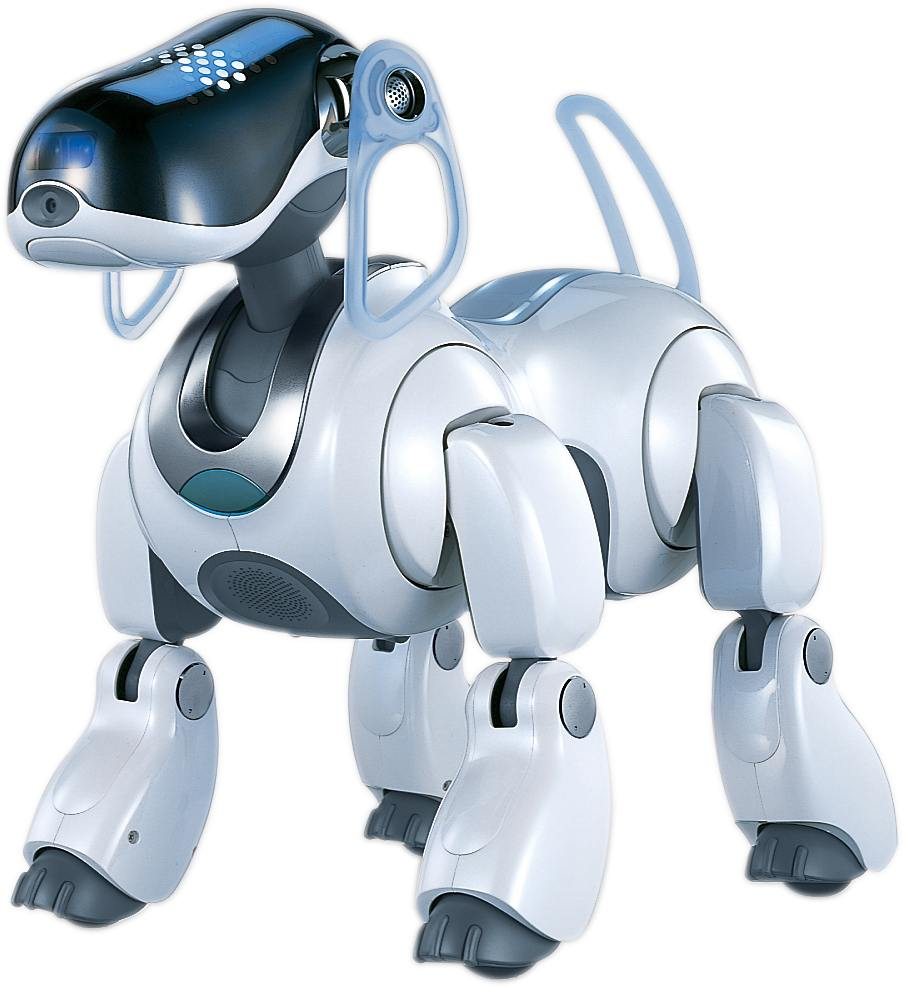
\includegraphics[scale=0.1]	{images/ers7lrg}
	 \caption{AIBO ERS-7.}
  \label{fig:ers7}
\end{figure}	
 
L'Aibo ERS-7 té les següents característiques\cite{morales}:
\begin{itemize}
\item Àudio:
\begin{itemize}
\item Entrada d'àudio: Micròfon estèreo
\item Sortida d'àudio: Altaveu de 20.8 mm i 500 mW
\end{itemize}
\item Sensors integrats:
\begin{itemize}
\item Sensors de pressió:
\begin{itemize}
\item 1 sobre el cap
\item 3 a l'esquena
\end{itemize}
\item 1 sensor de contacte a cada pota 
\item 1 sensor bolea sota la boca
\item Acceleròmetres en x,y i z
\item 2 sensors de proximitat d'infrarojos situats al morro i al pit
\item Sensor de vibració
\end{itemize}
\item Graus de llibertat
\begin{itemize}
\item 3 graus de llibertat a cada una de les 4 potes
\item 3 graus de llibertat al coll
\item 1 grau de llibertat a cada orella
\item 1 grau de llibertat a la boca
\item 2 graus de llibertat a la cua 
\end{itemize}
\item Entrada d'imatge
\begin{itemize}
\item Sensor d'imatge CMOS de 350000 píxels
\item Angles: 56.9º horitzontal i 45.2º vertical
\item Resolucions: 208x160, 104x80, 52x40
\item 30 frames per segon
\end{itemize}
\item Dimensions
\begin{itemize}
\item Altura: 278 mm
\item Llarg: 319 mm
\item Ample: 180 mm
\item Pes amb bateria: 1.65 Kg 
\end{itemize}
\item CPU:
\begin{itemize}
\item Processador: MIPS R7000 @ 576 MHz
\item RAM: 64 MB
\item Memòria flaix: 4 MB
\end{itemize}
\end{itemize}
\begin{itemize}
\item Connectivitat:
\begin{itemize}
\item LAN inalàmbric IEEE 802.11b
\item Xifrat: WEP
\end{itemize}
\end{itemize}

\subsection{El software}
APERIOS és el sistema operatiu en temps real que utilitzen els AIBO. APERIOS OS està destinat y dissenyat per poder treballar amb grans fluxos de dades d'àudio y d'imatge simultàniament en temps real.
En un inici AIBO va ser comercialitzat amb una finalitat purament lúdica, però degut al seu atractiu disseny i la seva robustesa va atreure l'atenció dels desenvolupadors per a convertir-se en una poderosa eina per a l'aprenentatge.Això va portar a Sony a publicar un API del seu sistema operatiu anomenada OPEN-R SDK. Arrel d'aquesta API van sorgir altres llenguatges i interfícies com son \textit{URBI}\footnote{\url{www.urbiforge.org}} o \textit{Tekkotsu}\footnote{\url{tekkotsu.org}} que posen una capa de programació per sobre de OPEN-R i permeten programar a més alt nivell.

\subsubsection{OPEN-R}
OPEN-R és un API en C++ que corre sobre el sistema APERIOS proporcionada per Sony i l'estructura de la cual és la que es mostra a la figura \ref{fig:openrarch}. OPEN-R diferencia entre dos nivells, la capa de sistema on s'accedeix al hardware del robot i la capa d'aplicació que es tracta dels programes fets per l'usuari.

\begin{figure}[h!]
	\centering
    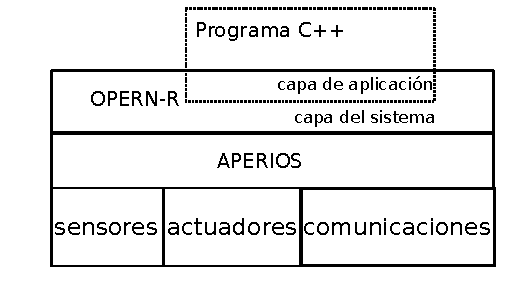
\includegraphics[scale=1]{images/openrarch.pdf}
	 \caption{Arquitectura de l'AIBO amb OPEN-R}
  \label{fig:openrarch}
\end{figure}


En tractar-se d'un llenguatge de baix nivell és inherent a l'estructura del sistema operatiu que es basa en objectes que interaccionen entre si mitjançant missatges o meta-objectes.El concepte d'objecte és semblant al utilitzat a \textit{UNIX}\footnote{\url{www.unix.org}} o a \textit{Windows}\footnote{\url{http://windows.microsoft.com/en-us/windows/home}}, amb la diferencia de que són mono-fil i que la comunicació és realitza per missatges que inclouen dades i un identificador que indica el metde en el que s'executarà en arribar a l'objecte destí. Això implica que cada objecte té varis punts d'entrada i sortida que són els mètodes: DoInit(), DoStart(), DoStop(), DoDestroy().
En el pas de missatges entre dos objectes, un d'ells es defineix com a subjecte(el que envia) i l'altre com observador(el que rep) qui inicia la seva execució després de que el missatge enviat faci saltar l'esdeveniment del mètode corresponent\cite{OPEN-R PG}.

\begin{table}[h]
\begin{center}
\begin{tabulary}{\textwidth}{|C|C|}
\hline
\multirow{1}{*}{\textbf{SUBJECTE}}
& \textbf{OBSERVADOR} \\ \hline
\multirow{1}{*}{enviament de dades}
& \\ \hline
\multirow{1}{*}{notificació de l'esdeveniment}
&  \\ \hline
\multirow{1}{*}{}
& recepció de dades \\ \hline
\multirow{1}{*}{}
& esdeveniment preparat  \\ \hline
\end{tabulary}
\end{center}
\caption{Estructura del pas de missatges a OPEN-R\label{msgOR}}
\end{table}
	
\begin{figure}[h!]
	\centering
    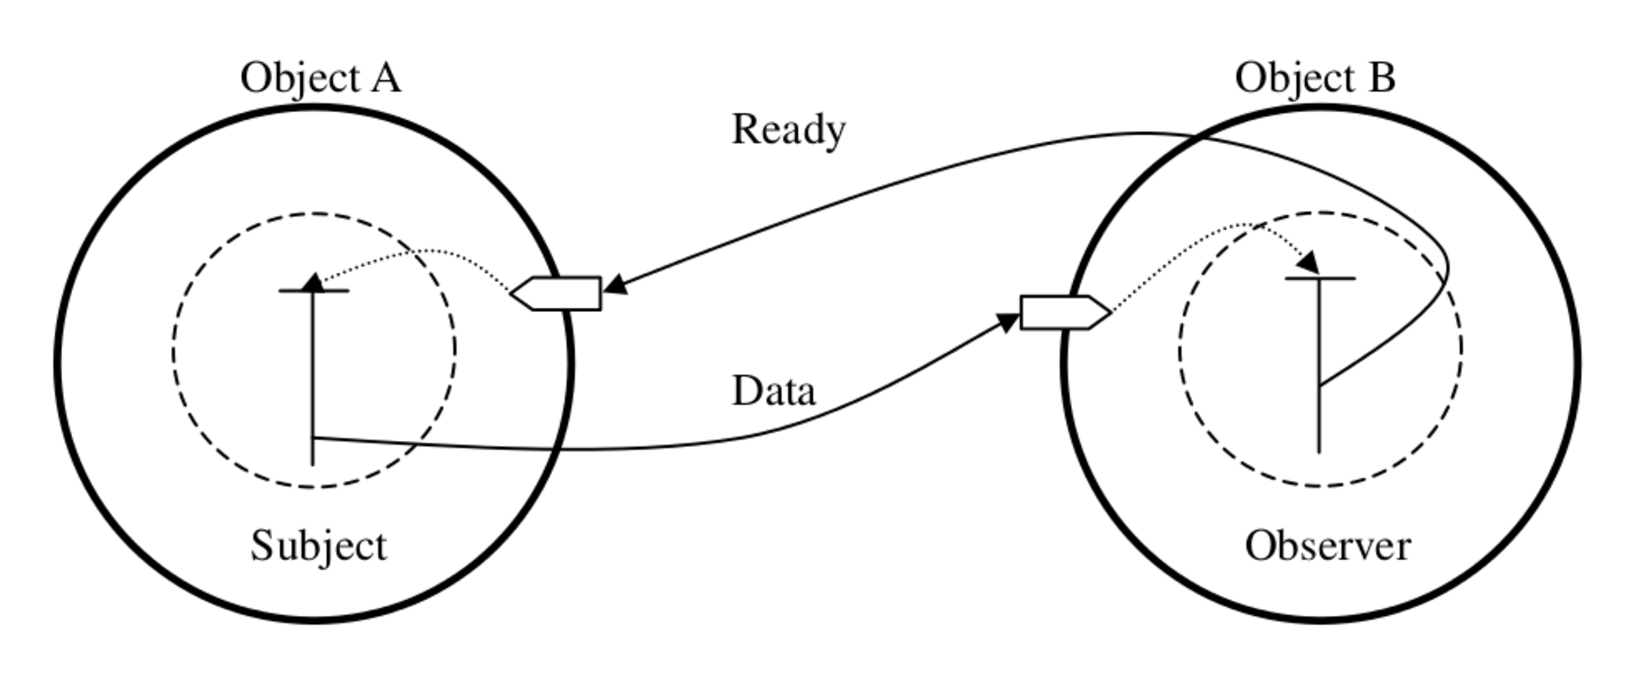
\includegraphics[scale=0.5]{images/ObjectCom.pdf}
	 \caption{Comunicació entre objectes.}
  \label{fig:objectcom}
\end{figure}

Una de les majors complicacións alhora de treballar amb OPEN-R és que treballa amb una gran varietat d'arxius que cal modificar per tal de configurar el programa d'aplicacio que es realitzi. Per aixó és important conèixer bé els arxius amb que es treballa, els més importants es troben llistats a continuació:
\begin{itemize}
\item Arxius .h i .cc: són els arxius de programació en C++.
\item STUB.config: són arxius de configuració on es defineix com l'objecte es comunica amb altres objectes.
\item Arxius .ocf: defineix el comportament dels objectes en quan a temps d'execució, memòria assignada i prioritat d'execució.
\item Makefile: és el fitxer per a la configuració global de compilació.
\item OBJECT.cfg: és el llistat d'objectes que s'executarà.
\item CONECT.cfg: on es determinen les connexions i comunicacions entre els objectes que s'executaran.
\item WLANCONFIG.txt\footnote{Aquest ultim archiu cal configurar-lo sigui quin sigui el mètode de programació del AIBO. Veure APENDIX} arxiu on es defineixen les característiques de la connexió inalàmbrica de l'AIBO.


\end{itemize}
\subsubsection{Tekkotsu}
Tekkotsu és una software de desenvolupament per a robots mobils. Originalment va ser creat per al robot AIBO de Sony, però actualment permet programar una amplia gama de robots com són el Chiara\footnote{\url{http://chiara-robot.org}}, iRobot Create\footnote{\url{http://chiara-robot.org/Create/}}, HandEye\footnote{\url{http://chiara-robot.org/HandEye/}} o Lynxmotion Arms\footnote{\url{http://www.lynxmotion.com/}}. Té una arquitectura basada en objectes i pas d'esdeveniments, igual que OPER-R fent un us complet de l'herència de C++. Proporciona una capa de major nivell que OPEN-R, però permet la crida a OPEN-R, el que significa que la capacitat de control sobre el robot és trobi limitada pel propi hardware i no per aquest software, permetent l'accés als sensors, complet control sobre els actuadors i la comunicacio basada en esdeveniments. Per altra banda permet a l'usuari poder treballar a alt nivell ja que el paquet inclou eines de processament visual bàsic, monitorització, models cinemàtica inversa i suport per a la creació de xarxes inalambriques. 

\begin{figure}[h!]
	\centering
    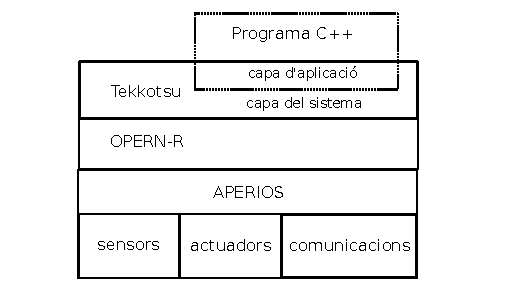
\includegraphics[scale=1.2]{images/tekk.pdf}
	 \caption{Arquitectura de l'AIBO amb tekkotsu.}
  \label{fig:tekk}
\end{figure}

A més Tekkotsu proporciona una interficie d'usuari, el ControllerGUI, que permet accedir al AIBO remotament i executar els comportaments que es desitgin i que estiguin programats a la targeta de memoria. Aixo tan es pot fer per la interficie grafica basada en java com per telnet\footnote{\url{http://es.wikipedia.org/wiki/Telnet}} al port 10020\cite{TekkQuickRef}.

Tekkotsu s'organitza com un conjunt de comportaments o "Behaviors" i classes MotionCommand. Les seves funcions s'executen en dos processos el "Main i el "Motion". En el primer s'encarrega de la percepció i la presa de decisions i el segon fa referencia al control en temps real dels actuadors. Existeix un tercer procés que s'encarrega de la sortida d'àudio\cite{tekkTut}. 

Igual que en OPEN-R, els comportaments, que son com s'anomena a qualsevol programa amb Tekkotsu, tenen una estructura basada en uns mètodes que cal respectar (doStart(), doStop()) que simplifica'n els 4 mètodes definits a OPEN-R, però que permeten mantenir l'estructura dels objectes i la comunicació entre ells basada en esdeveniments.  
 
\begin{figure}[h!]
	\centering
    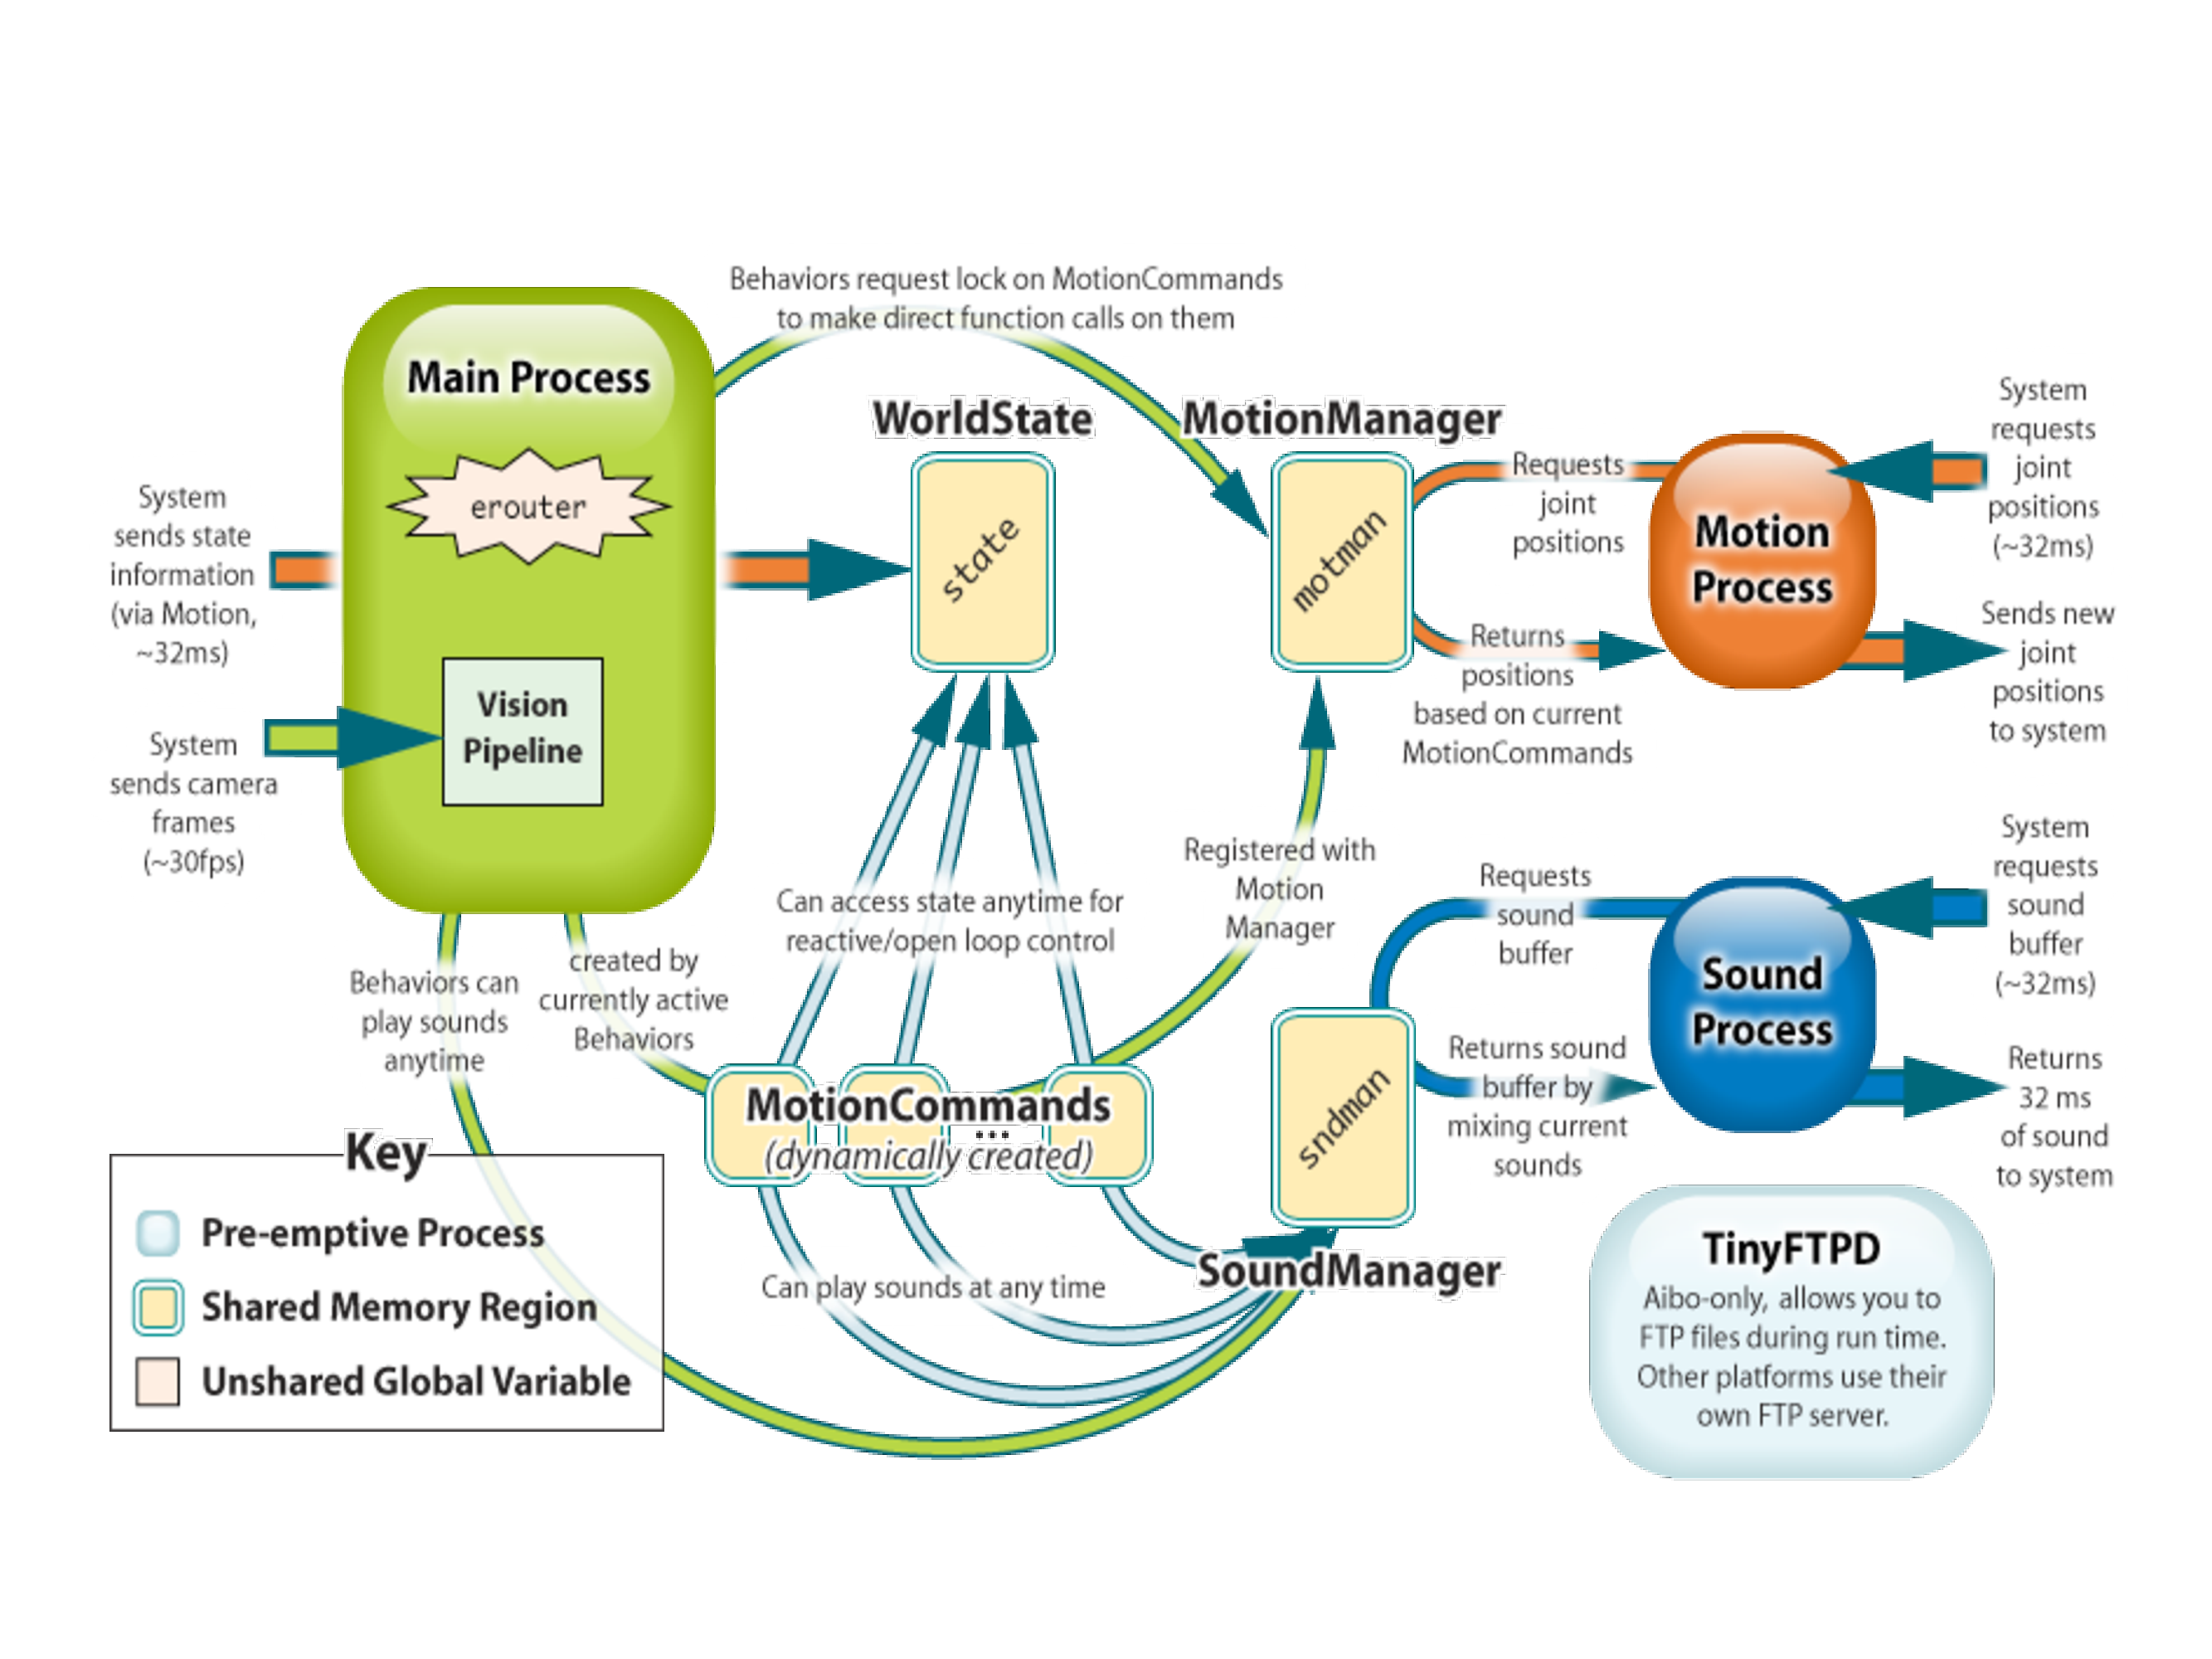
\includegraphics[scale=0.3]{images/tekkotsuarch.pdf}
	 \caption{Procés d'execució d'un programa amb Tekkotsu.}
  \label{fig:tekkarch}
\end{figure}

\subsubsection{URBI}
\label{urbi}
URBI és l'acrònim de Universal Real-Time Behavior Interface i es tracta d'una plataforma de software lliure per controlar robots i sistemes complexos en general com AIBO, Bioloid\, Mindstorm NXT, Pioneer, Wifibot o ARDrone\cite{urbi}. URBI és un llenguatge basat en scripts d'alt nivell amb l'avantatge de que permet executar comandes en paral·lel. per treballar amb URBI existeixen dos maneres, una es tracta d'utilitzar el script per després incloure un objecte d'OPEN-R a la targeta de memoria de l'AIBO que el propi sistema operatiu APERIOS pot interpretar i executar. La segona manera consisteix en una arquitectura client/servidor on el servidor es tracta com un objecte OPEN-R que va dins del robot i el client envia comandes que son executades per el servidor, Figura \ref{fig:urbiarc}. 

\begin{figure}[h!]
	\centering
    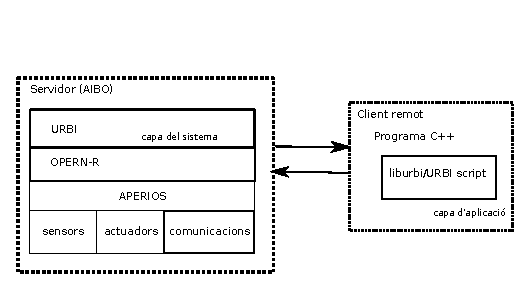
\includegraphics[scale=1.4]{images/urbiarc.pdf}
	 \caption{Arquitectura de l'AIBO amb URBI.}
  \label{fig:urbiarc}
\end{figure}

Aquesta segona opció obre varies vies per a la programació. Permet, per una banda comunicar-se per telnet i enviar les comandes o bé usar la llibreria liburbi que permet treballar amb C++, Java i Matlab o varis llenguatges alhora mitjançant varis clients.
URBI permet i facilita l'accés a cada una de les articulacions i sensors de l'AIBO, per exemple per consultar el valor de la primera articulació de la cama esquerre del devant cal enviar la comanda \texttt{legLF1.val;} i per assignar el seu valor \texttt{legLF1.val=20;}\cite{urbicmd}. A l'apèndix\ref{urbiA} és pot trobar més documentació sobre les comandes d'URBI.

\clearpage
\section{Comparació d'alternatives per a la programació}

Tenint en conte que el que és preten és buscar una forma senzilla i rapida de enviar l'estat dels sensors i articulacions de l'AIBO a un PC remot i enviar a l'AIBO les posicions desitjades de les articulacions per tal de poder treballar posteriorment amb ROS s'han tingut en conte certes consideracions qualitatives un trobades durant la recerca que es troben resumides a la Taula \ref{complleng}.

En els tres casos és necessari programar amb el llenguatge corresponent per al client del PC. A excepció de Urbi seria necessari desenvolupar un programa per a l'AIBO de manera que permetés enviar i rebre les dades necessaries. Amb Urbi no és necessari ja que la llibreria liburbi permet accedir a totes les dades necessaries i també ho permet fer per telnet. Tekkotsu, en canvi, permet obtenir els valors de sensors i actuadors per telnet però no actuar sobre ells, caldria doncs un comportament que implementés aquest fet. De totes formes amb Tekkotsu hi han hagut problemes per tal de trobar documentació ja que s'ha trobat per a la versió més nova Tekkotsu 5.1 i tot i que Tekkotsu va neixer arrel de l'AIBO aquesta versió sembla no ser compatible amb el ultim OPEN-R SDK. La unica versió que s'ha conseguit compilar i la única trobada apart de la 5.1 és la 4.0.1 de la qual no s'ha trobat cap mena de documentació i d'una a l'altre canvia el mètode de programació.
Pel que respecte a R-CODE seria una bona opció ja que es parteix de més baix nivell i per a l'objectiu d'aquest projecte això és un incentiu, però cal invertir molt de temps en l'aprenentatge del llenguatge. 


\begin{table}[h]
\begin{center}
\begin{tabulary}{\textwidth}{|p{5cm}|p{2.5cm}|p{2.5cm}|p{2.5cm}|}
\hline

& \textbf{OPEN-R}
& \textbf{Urbi} 
& \textbf{Tekkotsu} \\\hline
Necessitat de un programa a l'AIBO
& Si
& No
& Si \\ \hline
Necessitat d'un programa al PC
& Si
& Si
& Si\\ \hline
Permet consultar l'estat per telnet
& No
& Si
& Si\\ \hline
Permet accionar articulacions per telnet
& No
& Si
& No\\ \hline
Dificultat de programació (0-5)
& 5
& 2 
& 3\\ \hline
Documentació (0-5)
& 2
& 3
& 1\\ \hline
Plataforma del PC
& Windows/ Linux/ OS
& Windows/ Linux 32bits/ OS
& Linux\\ \hline
\end{tabulary}
\end{center}
\caption{Comparació entre llenguatges usats en l'AIBO\label{complleng}}
\end{table}

Per aquests motius s'ha decidit partir de dos opcions per a desenvolupar el paquet de ROS que permetrà controlar l'AIBO.

La primera s'usara liburbi en un programa C++ i la segona es provarà de fer la comunicació amb un script de python usant una connexió telnet.

\subsection{Lectura de dades}
En un primer experiment per comparar les possibles solucions s'ha realitzat la lectura d'una variable del sistema per tal de valorar quantitativament la velocitat de transmissió. S'ha usat el valor de la posició d'una articulació.

El procediment per a l'adquisició de dades serà el mostrat a la Taula \ref{readleg}.
\begin{table}[h]
\begin{center}
\begin{tabulary}{\textwidth}{|C|C|}
\hline
\multirow{1}{*}{\textbf{CLIENT}}
& \textbf{SERVIDOR} \\ \hline
\multirow{1}{*}{demanda d'inici del bucle d'enviament}
& \\ \hline
\multirow{1}{*}{lectura de les dades}
& enviament de dades \\ \hline
\multirow{1}{*}{Escriptura en archiu extern}
&  enviament de dades \\ \hline

\end{tabulary}
\end{center}
\caption{Estructura de la lectura d'una variable\label{readleg}}
\end{table}

Es consulta el temps en el que es rep cada dada reben aquest temps amb precisió de nanosegons i escribint-lo   en un archiu de text per al seu posterior tractament.

Es realitzen 15 repliques per a cada cas i cada una d'elles tindrà una durada de 10 segons per tal de poder estimar de forma precisa quina és la millor opció per tal de rebre les dades de L'AIBO.

\subsubsection{Metode amb liburbi i C++}

Usant la llibreria liburbi es tracta d'enviar per un client urbi la comanda per tal de rebre les dades de la primera articulació de la cama esquerre. 
L'estructura del programa és la que segueix\footnote{El script es pot trobar a l'annexe \ref{getDataOneLegC++}}.
\begin{itemize}
\item Inicialitzacó del client URBI.
\item Inicialització del callback. 
Aquest serà cridat cada cop que es rebi una dada per a l'etiqueta assignada.
\begin{itemize}
\item Es pren el valor de la variable (tot i que per aquest experiment no es necessiti.).
\item Es consulta el temps en que ha estat rebuda aquesta dada.
\item Es guarda la dada i el temps.
\end{itemize}
\item Demanda del bucle i assignació a una etiqueta.
\item Inicialització del archiu on es guradaràn les dades.
\item  Execució del bucle de urbi. 
\end{itemize}



%\texttt{loop legLF1 << legLF1.val,}
\subsubsection{Metode amb telnet i python}
La idea d'aquest script\footnote{Es pot cunsultar el script a lannexe \ref{getDataOneLegPy}} es treballar amb urbi com si fos la una terminal de urbi \ref{fig:telnet} però mitjançant python per tant l'estructura bàsica serà enviar la comanda i llegir la resposta per a que pugui ser tractada. 
\begin{figure}[h!]
	\centering
    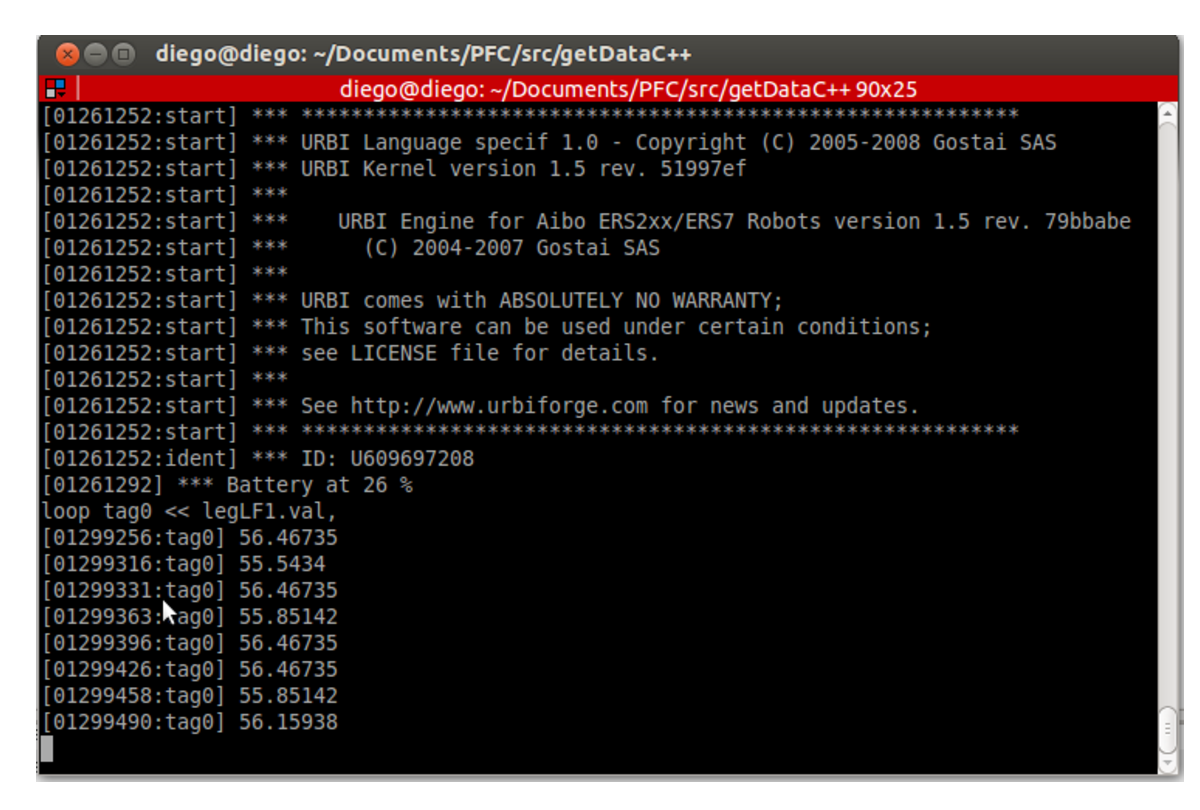
\includegraphics[scale=0.65]{images/telnet.pdf}
	 \caption{terminal de Urbi consultant dades.}
  \label{fig:telnet}
\end{figure}
Així doncs l'estructura serà semblant al script de C++:
\begin{itemize}
\item Inicialització de l'objecte telnet.
\item Petit retràs per esperar la connexió.
\item Lectura i eliminació de la capsalera del terminal urbi rebuda pel terminal.
\item Escriptura de la comanda del bucle d'enviament del valor de l'articulació més una variable concreta per facilitar una marca per al tractament de les dades rebudes.
\item Bucle de lectura i escriptura.
\begin{itemize}
\item Tractament de les dades:
\begin{itemize}
\item Lectura fins a trobar la marca.
\item Eliminació de les cadenes rebudes tallades per la informació de la bateria\footnote{Cada poc temps la terminal de urbi escriu el percentatge de bateria restant.}
\item Separació de la cadena de caràcters per agafar únicament el valor de l'articulació.
\
\end{itemize}
\item Escriptura de la dada a l'arxiu.
\item Adquisició del temps.
\item Escriptura del temps a l'arxiu.
\end{itemize} 
\end{itemize}



\subsubsection{Comparacó}

Dels programes anteriorment explicats s'obtenen les 15 repliques de 10 segons cada una. Dels temps extrets s'obté l'invers de les diferències de temps entre dades rebudes, doncs és més intuïtiu i per analitzar el trafic i la velocitats de dades es preferible treballar amb Hertz que amb el seu invers.

Graficant les dades a les Figures \ref{fig:OneLegC++Box} i \ref{fig:OneLegPythonBox} s'observa com la variabilitat dels resultats, dins de cada rèplica, del cas en que s'usa liburbi és més alta, però també els valors semblen ser considerablement més alts. 

\begin{figure}[H]
	\centering
    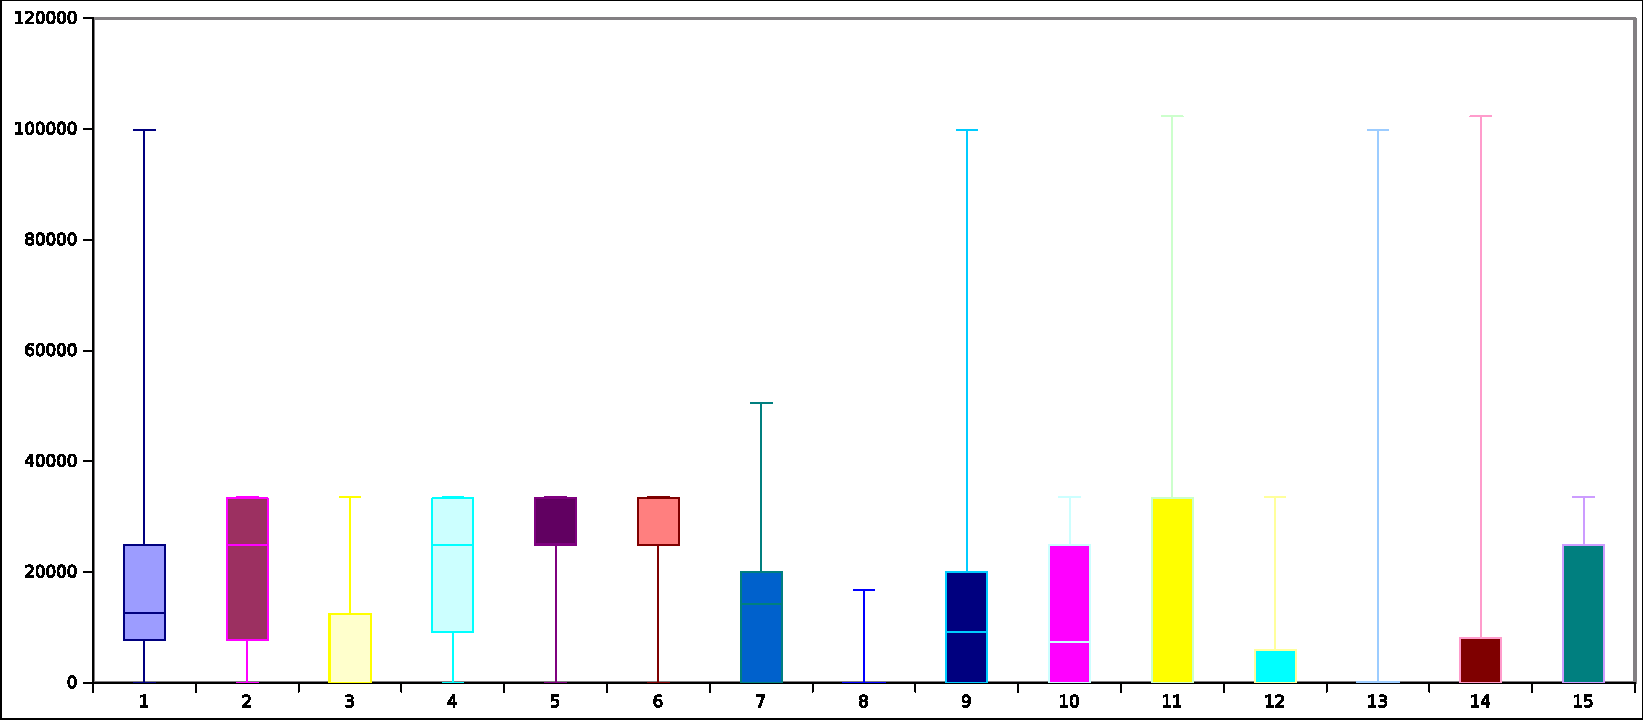
\includegraphics[scale=0.5]{images/OnelegC++Box.pdf}
	 \caption{Diagrama de caixa de la freqüència de dades per a les 15 repliques de l'experiment amb liburbi.}
  \label{fig:OneLegC++Box}
\end{figure}

\begin{figure}[H]
	\centering
    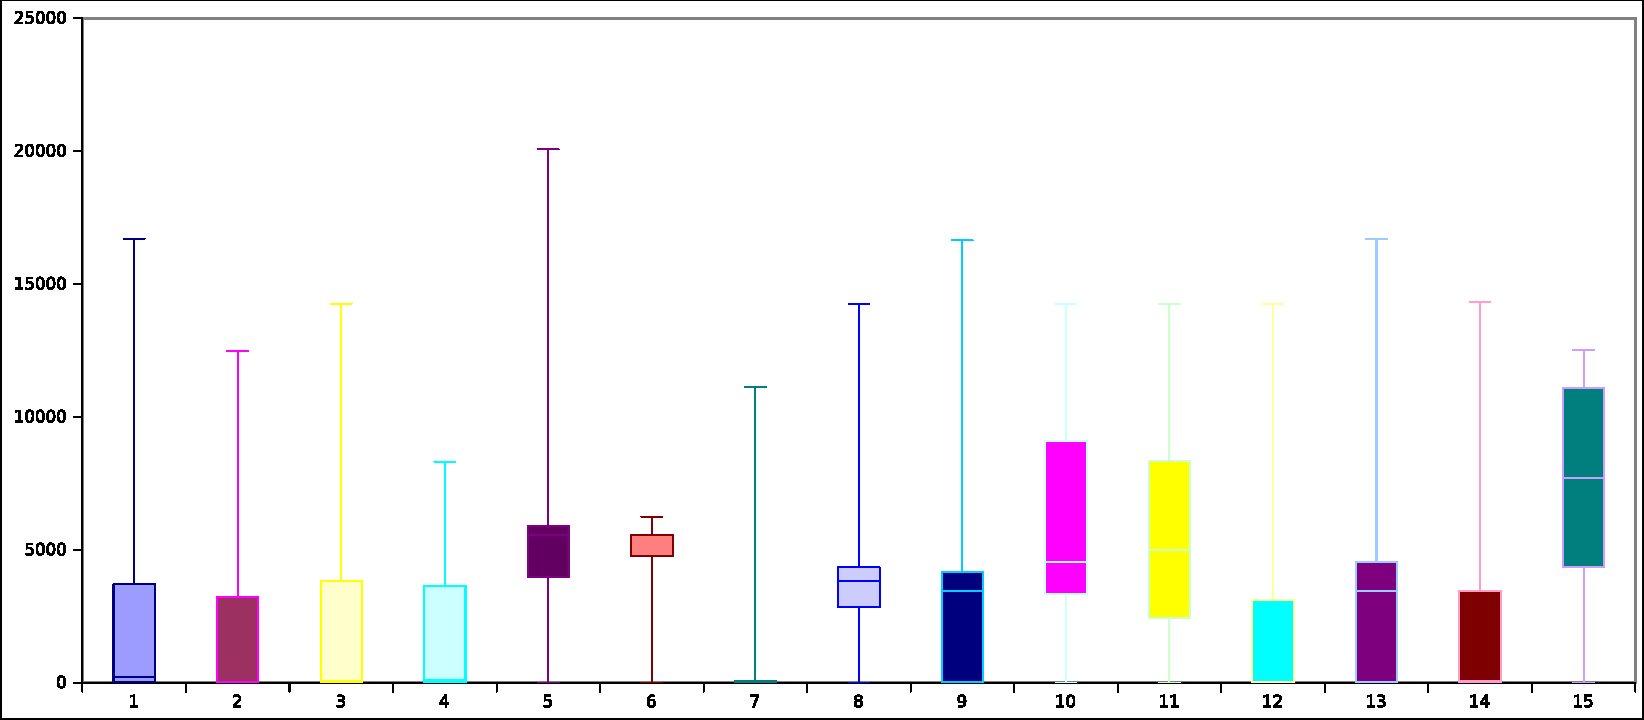
\includegraphics[scale=0.5]{images/OneLegPythonBox.pdf}
	 \caption{Diagrama de caixa de la freqüència de dades per a les 15 repliques de l'experiment amb telnet.}
  \label{fig:OneLegPythonBox}
\end{figure}

Per corroborar aquests dos fets s'ha pres una serie de variables característiques de cada mostra. Les Figures \ref{fig:DevOneLeg} i \ref{fig:MitOneLeg} mostren de forma més visual aquest fet i permeten afirmar que el primer cas  te una velocitat de transmissió de dades mitja més elevat, però la seva variabilitat també és significativament major.

\begin{figure}[H]
	\centering
    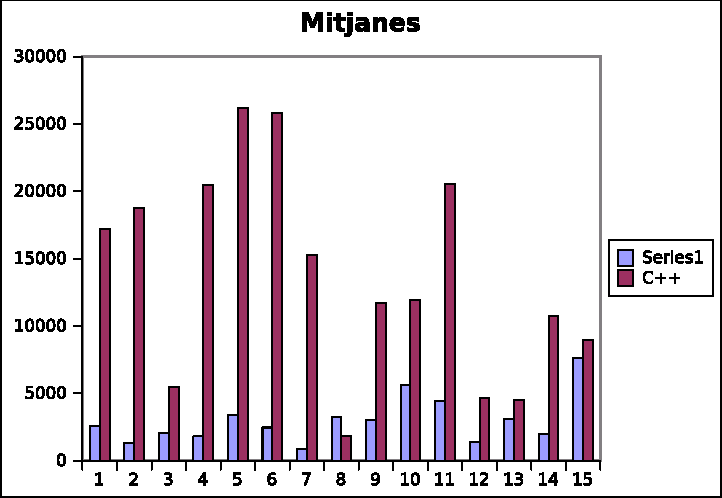
\includegraphics[scale=1]{images/mitjanesOneLeg.pdf}
	 \caption{Freqüència mitjana en Hz de les 15 repliques de cada mètode.}
  \label{fig:MitOneLeg}
\end{figure}
\begin{figure}[H]
	\centering
    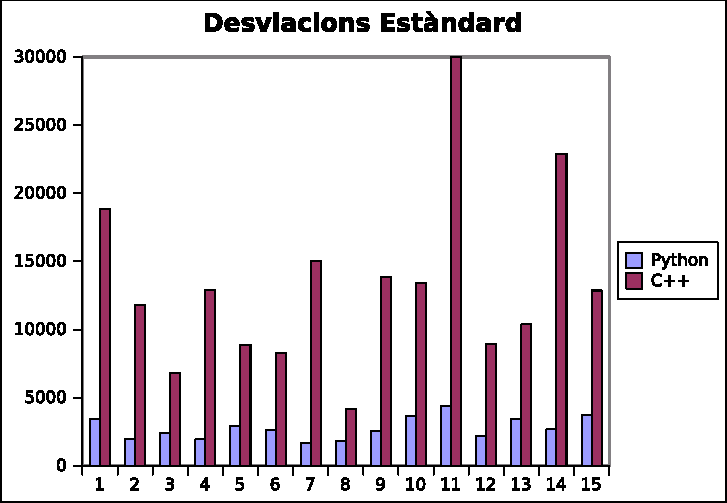
\includegraphics[scale=1]{images/DevOneLeg.pdf}
	 \caption{Desviacions estàndard de la freqüència en les 15 repliques dels dos mètodes.}
  \label{fig:DevOneLeg}
\end{figure}

Tanmateix no és sols la velocitat mitja el que interessa sinó que sigui suficientment constant i sobre tot que els temps de congelació en el refresc d'una variable siguin el mes petit possible.
Observant doncs les freqüències mínimes Figura\ref{fig:MinOneLeg} no sembla que en algun dels dos casos aquestes siguin inferiors altres. Si bé es cert que els buits més grans es donen amb liburbi realitzant un anàlisi sobre la variança (ANOVA) no es pot afirmar que en aquest aspecte siguin poblacions diferents. 

\begin{figure}[H]
	\centering
    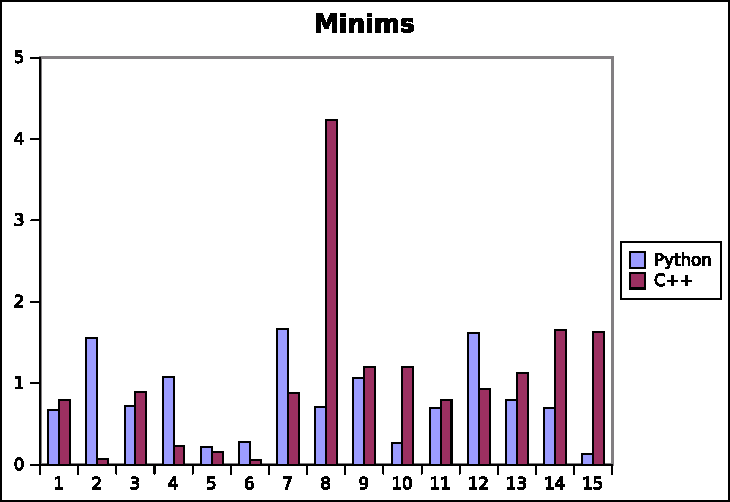
\includegraphics[scale=1]{images/MinOneLeg.pdf}
	 \caption{Mínims de la freqüència en les 15 repliques dels dos mètodes.}
  \label{fig:MinOneLeg}
\end{figure}

En vista dels resultats obtinguts s'ha volgut comprovar com afecta el nombre de dades en els temps de recepció de les variables. Per això s'ha realitzat el mateix experiment però en comptes de llegir únicament el valor d'una articulació, s'envien els valors de totes les articulacions.

Els resultats obtinguts en diagrames de caixes Figures \ref{fig:JointsC++Box} i \ref{fig:JointsPythonBox} mostren com les dos mostres son més semblants entre els dos casos. El temps maxim d'adquisició de dades del metode amb telnet ha incrementat fins a igualarse amb el de liburbi. La diferència pot ser que amb aquest mètode es rep una trama que es tracta en paral·lel a la recepció de dades mentre que el cas de liburbi es un sol callback que es va disparant per a cada valor i per tant el cas de telnet li costarà el mateix rebre totes les dades que una mentre que amb liburbi no.



\begin{figure}[H]
	\centering
    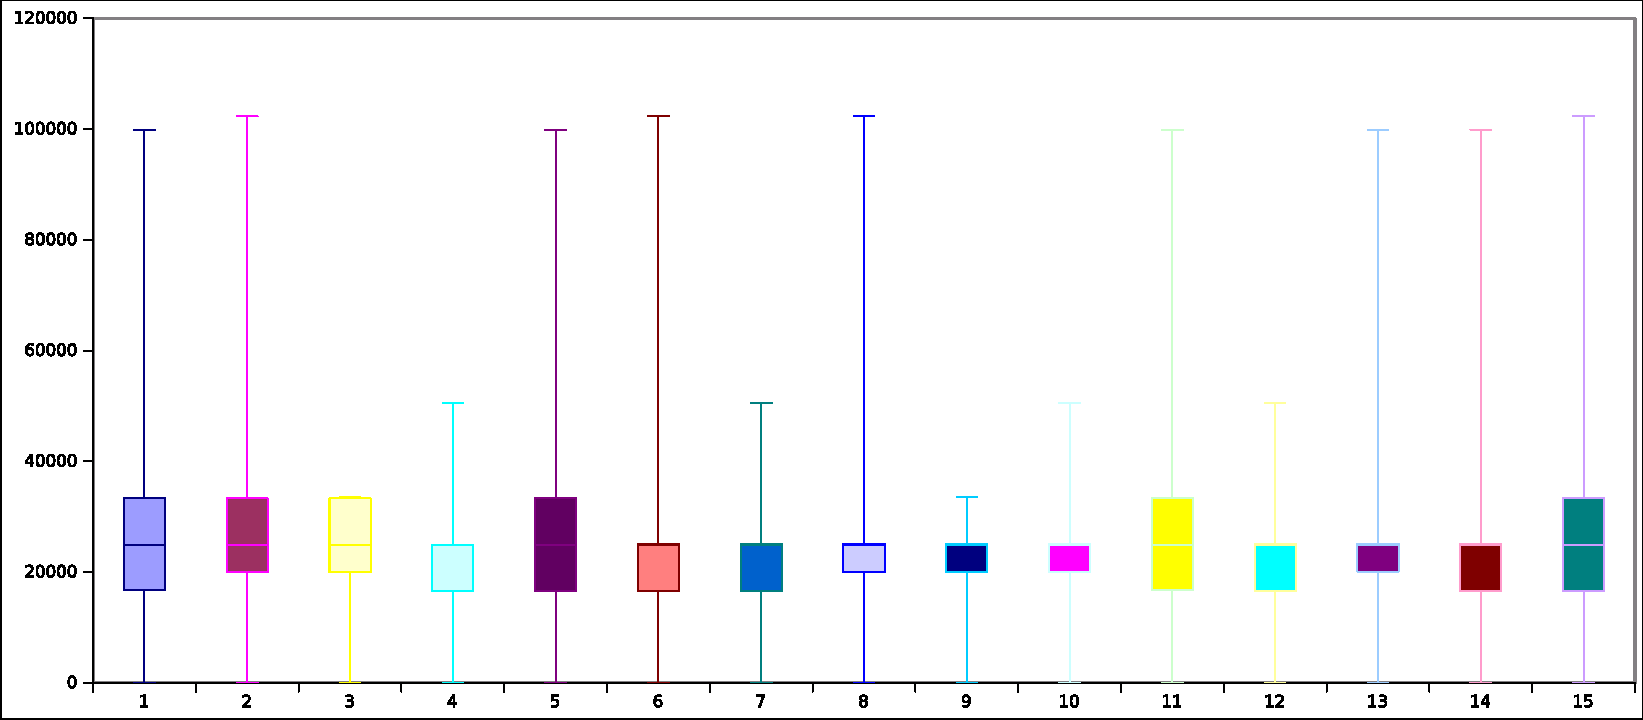
\includegraphics[scale=0.5]{images/JointC++Box.pdf}
	 \caption{Diagrama de caixa de la freqüència de dades per a les 15 repliques de l'experiment amb liburbi.}
  \label{fig:JointsC++Box}
\end{figure}
\begin{figure}[H]
	\centering
    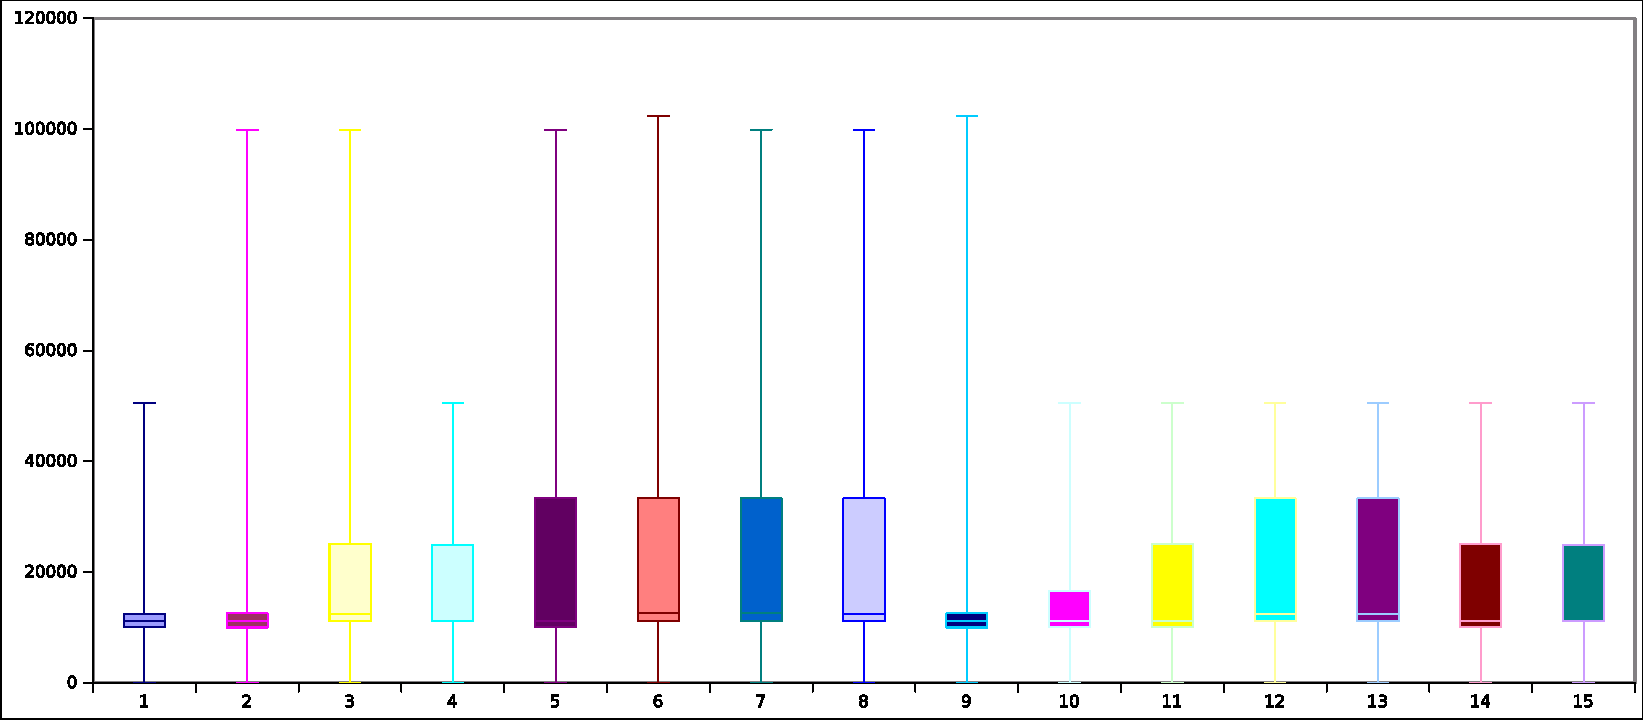
\includegraphics[scale=0.5]{images/JointsPythonBox.pdf}
	 \caption{Diagrama de caixa de la freqüència de dades per a les 15 repliques de l'experiment amb telnet.}
  \label{fig:JointsPythonBox}
\end{figure}

Les mitjanes semblen lleugerament més altes les del programa de liburbi Figura\ref{fig:MitJoint} tot i que no hi ha les diferències de l'experiment anterior i pel que fa a les desviacions seblen força semblants.


\begin{figure}[H]
	\centering
    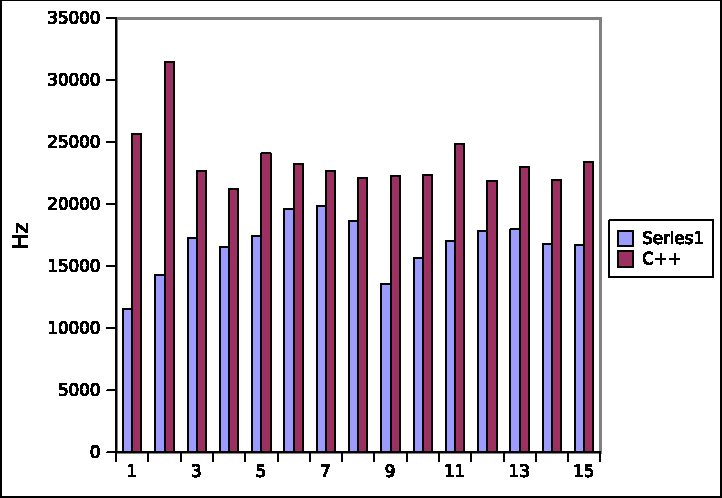
\includegraphics[scale=1]{images/MitJoint.pdf}
	 \caption{Freqüència mitjana en Hz de les 15 repliques de cada mètode.}
  \label{fig:MitJoint}
\end{figure}
\begin{figure}[H]
	\centering
    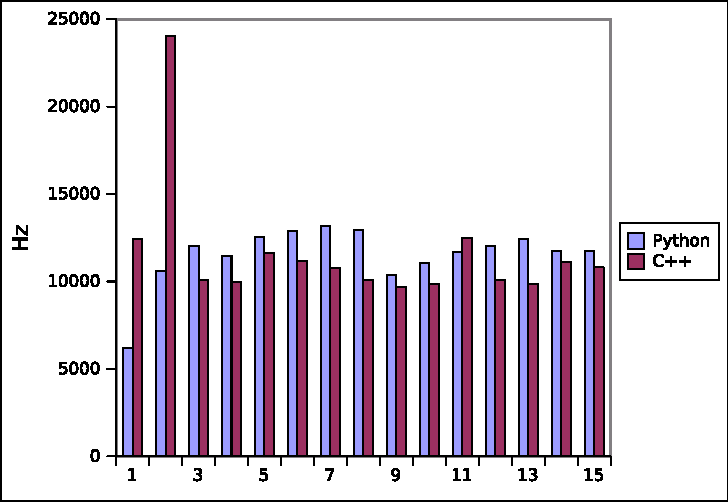
\includegraphics[scale=1]{images/DevJoint.pdf}
	 \caption{Desviacions estàndard de la freqüència en les 15 repliques dels dos mètodes.}
  \label{fig:DevJoint}
\end{figure}
Fixants en les frequencies mínimes sembla que els dos tenen un comportament semblant. Comparant aquests valors amb una ANOVA es pot veure que efecitivament no es poden considerar poblacions diferents.
\begin{figure}[h!]
	\centering
    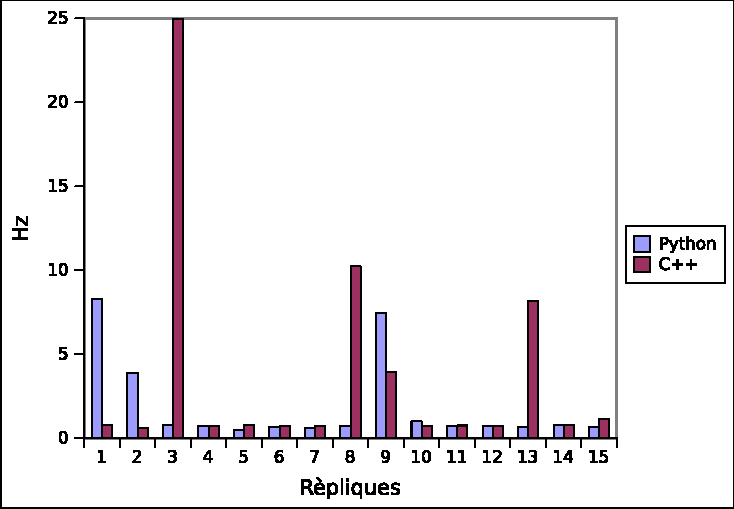
\includegraphics[scale=1]{images/MinJoint.pdf}
	 \caption{Mínims de la freqüència en les 15 repliques dels dos mètodes.}
  \label{fig:MinJoint}
\end{figure}
%
%\begin{table}[h]
%\begin{center}
%\begin{tabulary}{\textwidth}{|c|c|c|c|c|}
%\hline
%
%\textbf{Replica} & \textbf{Mitjana} & \textbf{Desviació estàndard} & \textbf{Màxim} & \textbf{Minim} \\ \hline
%1 & 17220.69 & 18868.55 & 99864.38 & 0.8  \\ \hline
%2 & 18751.08 & 11781.05 & 33554.43 & 0.07  \\ \hline
%3 & 5478.21 & 6845.21 & 33554.43 & 0.9  \\ \hline
%4 & 20500.1 & 12917.91 & 33554.43 & 0.23\\ \hline
%5 & 26177.68 & 8864.36 & 33554.43 & 0.16\\ \hline
%6 & 25822.19 & 8260.97 & 33554.43 & 0.06\\ \hline
%7 & 15288.78 & 15038.49 & 50533.78 & 0.88 \\ \hline
%8 & 1826.91 & 4198.85 & 16710.37& 4.24 \\ \hline
%9 & 11732.41 & 13836.05 & 99864.38 & 1.2\\ \hline
%10 & 11941.76 & 13410.92 & 33554.43 & 1.2\\ \hline
%11 & 20545.05 & 29980.55 & 102300.1 & 0.8\\ \hline
%12 & 4640.01 & 8933.51 & 33554.432& 0.93 \\ \hline
%13 & 4520.6 & 10376.95 & 99864.38 & 1.13 \\ \hline
%14 & 10729.39 & 22888.43 & 102300.1 & 1.66\\ \hline
%15 & 8989.98 & 12864.7 & 33554.43 & 1.64 \\ \hline
%\end{tabulary}
%\end{center}
%\caption{dades de C++\label{onelegC++}}
%\end{table}
%\begin{table}[h]
%\begin{center}
%\begin{tabulary}{\textwidth}{|c|c|c|c|c|}
%\hline
%
%\textbf{Replica} & \textbf{Mitjana} & \textbf{Desviació estàndard} & \textbf{Màxim} & \textbf{Minim} \\ \hline
%1 & 17220.69 & 18868.55 & 99864.38 & 0.8  \\ \hline
%2 & 18751.08 & 11781.05 & 33554.43 & 0.07  \\ \hline
%3 & 5478.21 & 6845.21 & 33554.43 & 0.9  \\ \hline
%4 & 20500.1 & 12917.91 & 33554.43 & 0.23\\ \hline
%5 & 26177.68 & 8864.36 & 33554.43 & 0.16\\ \hline
%6 & 25822.19 & 8260.97 & 33554.43 & 0.06\\ \hline
%7 & 15288.78 & 15038.49 & 50533.78 & 0.88 \\ \hline
%8 & 1826.91 & 4198.85 & 16710.37& 4.24 \\ \hline
%9 & 11732.41 & 13836.05 & 99864.38 & 1.2\\ \hline
%10 & 11941.76 & 13410.92 & 33554.43 & 1.2\\ \hline
%11 & 20545.05 & 29980.55 & 102300.1 & 0.8\\ \hline
%12 & 4640.01 & 8933.51 & 33554.432& 0.93 \\ \hline
%13 & 4520.6 & 10376.95 & 99864.38 & 1.13 \\ \hline
%14 & 10729.39 & 22888.43 & 102300.1 & 1.66\\ \hline
%15 & 8989.98 & 12864.7 & 33554.43 & 1.64 \\ \hline
%\end{tabulary}
%\end{center}
%\caption{dades de C++\label{onelegPython}}
%\end{table}

\subsection{Enviament de dades}
Part de la comunicació te a veure amb l'enviament de ordres a les articulacions del AIBO, amb aquest motiu s'ha realitzat un altre experiment. 
Aquest consistirà en enviar variar de forma sinusoïdal el valor d'una articulació mentre es llegeixen els valors de les articulacions com a l'apartat anterior. 
En aquest cas tenim 3 opcions de programació: liburbi usant solament un client, liburbi usant un client per llegir i laltre per escriure i finalment per telnet.
En els tres casos ha sigut necessària la creació d'un altre fil d'execució per poder dur a terme la lectura i la escriptura en paral·lel\footnote{Els codis es poden trobar a l'annex \ref{sinC} i \ref{sinP}}.
L'experiment s'ha realitzat a diverses freqüències a la que s'enviaven els punts de la sinusoide. S'ha realitzat per a 1, 2, 5 i 10 Hz no s'ha enviat a més freqüència degut a que el moviment resultant a 10 Hz començava a ser poc suau i inconstant. A més s'ha pogut comprovar que a més freqüència el buffer d'entrada d'ordres de l'AIBO sembla que es bloqueja.  
\begin{figure}[H]
	\centering
    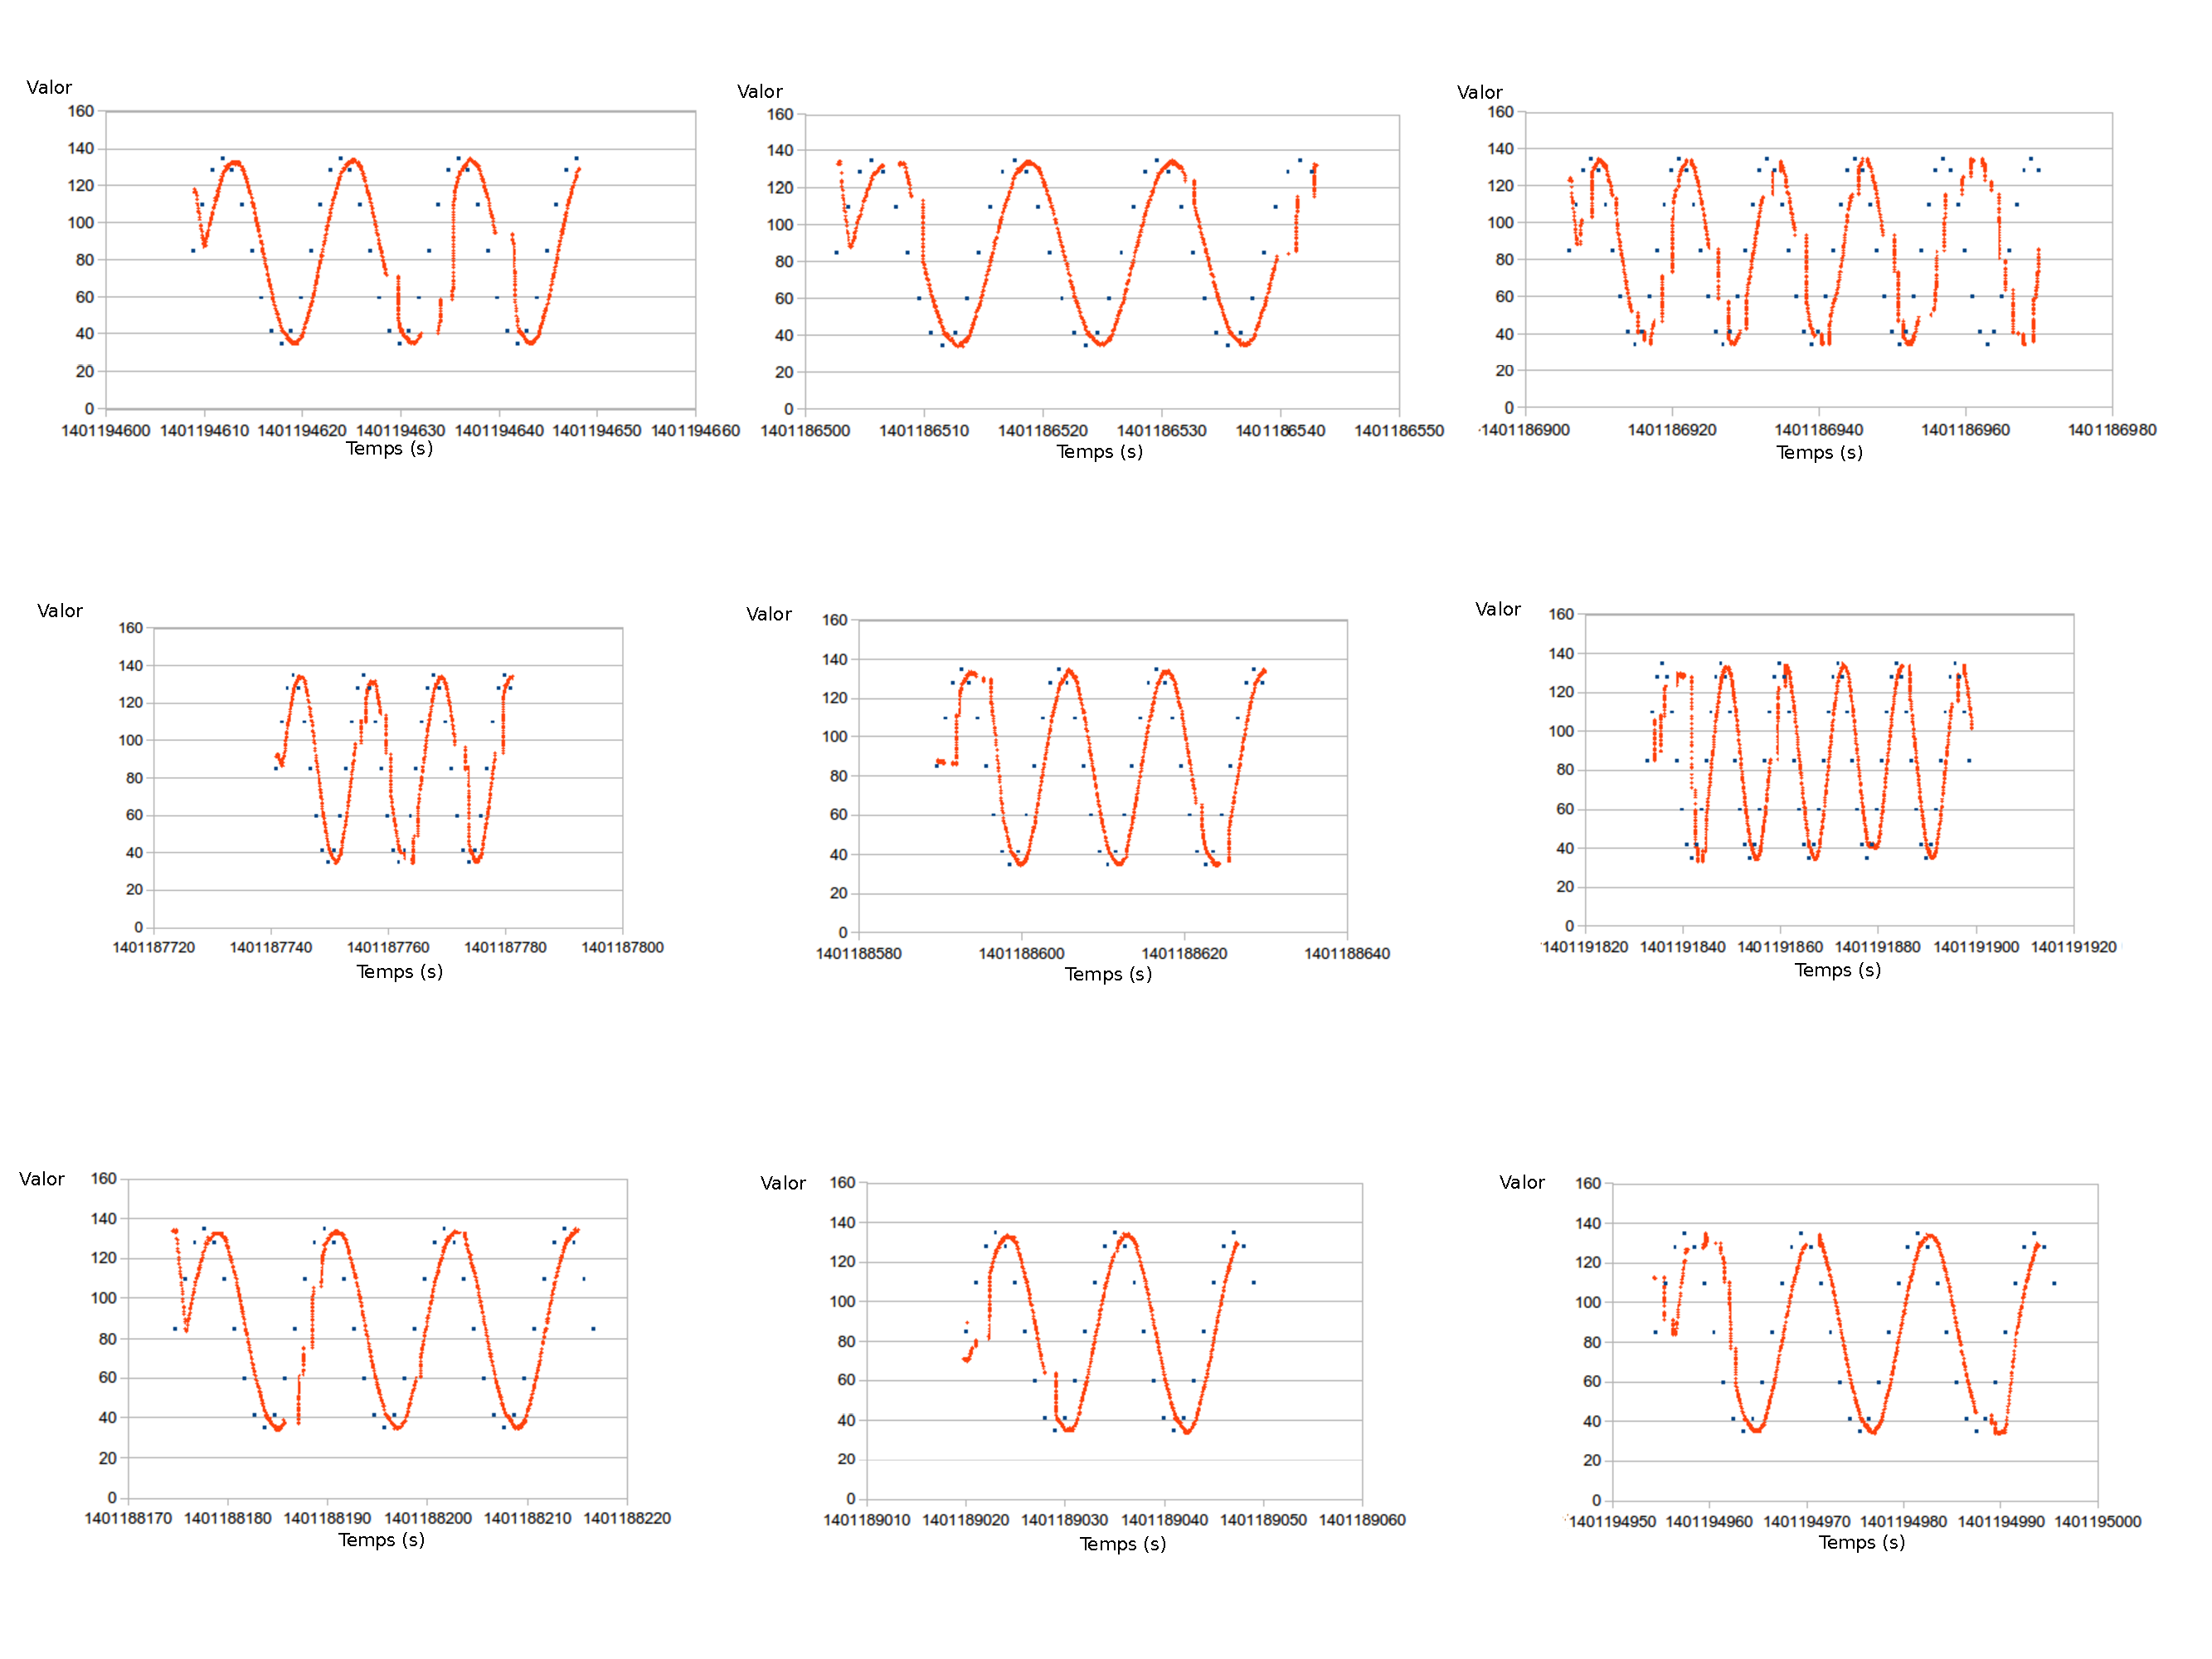
\includegraphics[scale=0.33]{images/sin1H.pdf}
	 \caption{En blau està graficat les posicions enviades a una freqüència d'1Hz i en vermell les lectures realitzades. En columnes es troben les repliques del mateix experiment i per files els tres mètodes usats, començant per liburbi amb un client, liburbi amb dos clients i telnet.}
  \label{fig:sin1H}
\end{figure}
\begin{figure}[H]
	\centering
    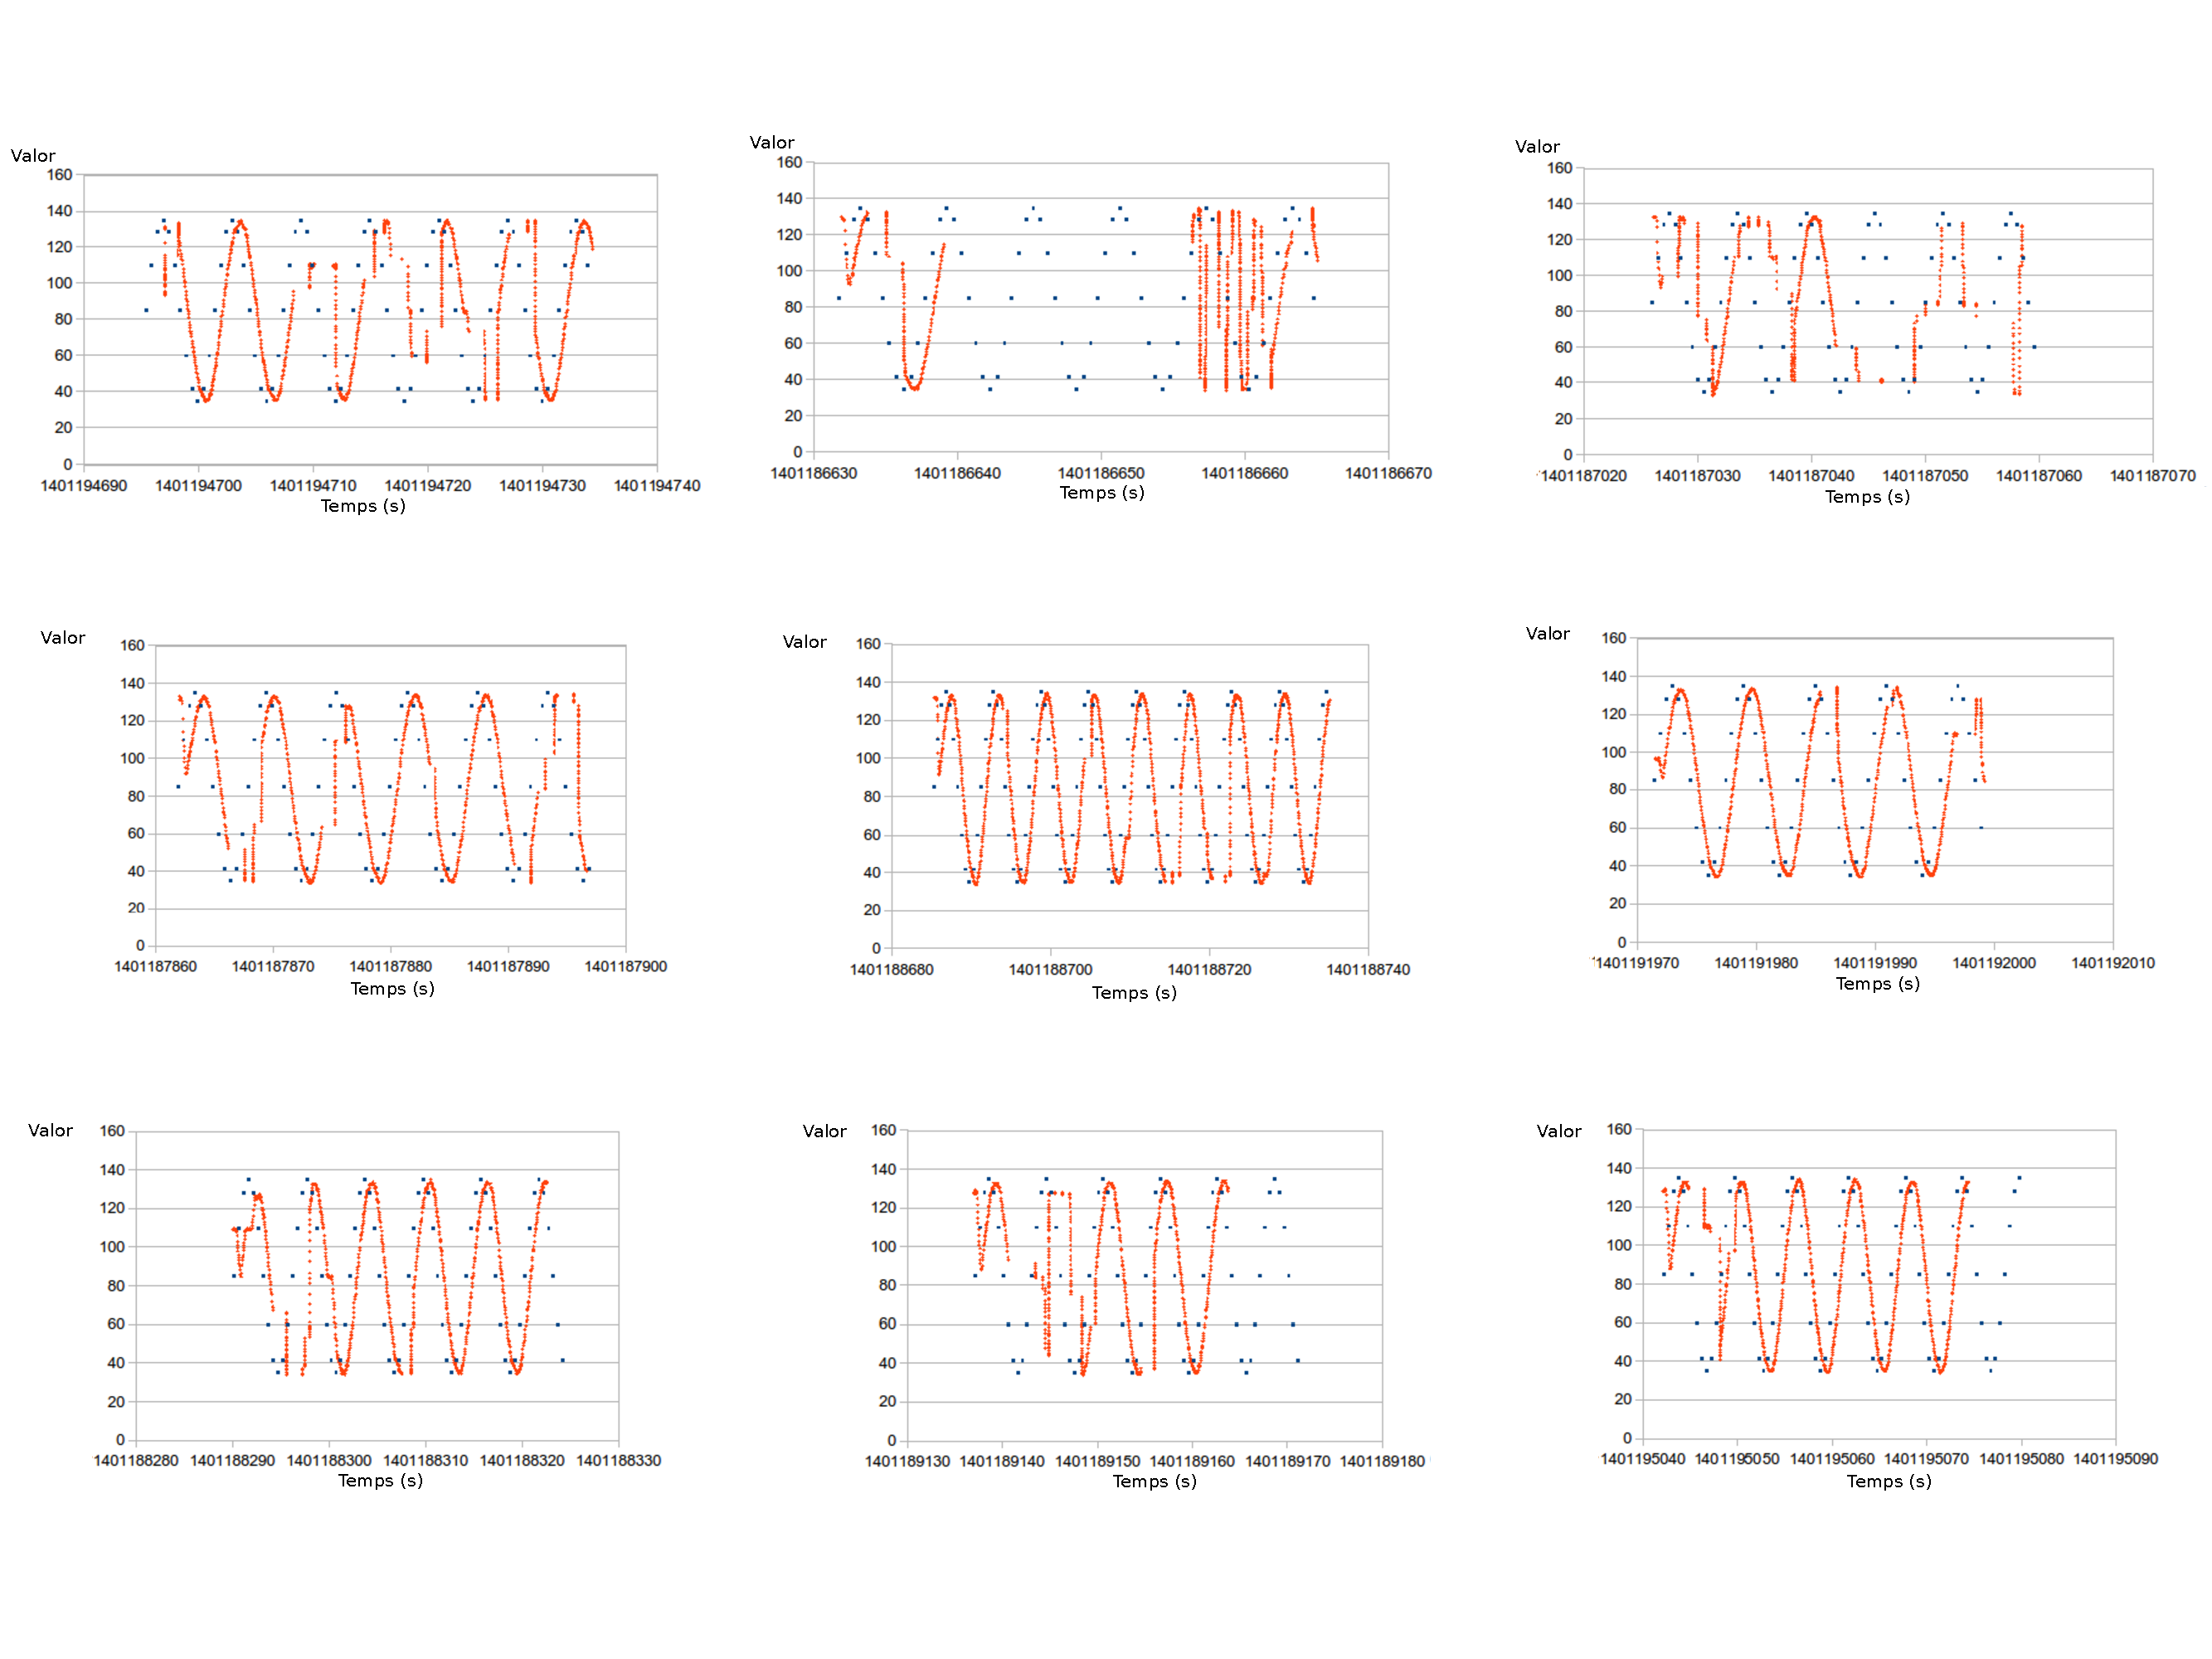
\includegraphics[scale=0.3]{images/sin2H.pdf}
	 \caption{En blau està graficat les posicions enviades a una freqüència d'2Hz i en vermell les lectures realitzades. En columnes es troben les repliques del mateix experiment i per files els tres mètodes usats, començant per liburbi amb un client, liburbi amb dos clients i telnet.}
  \label{fig:sin2H}
\end{figure}
\begin{figure}[H]
	\centering
    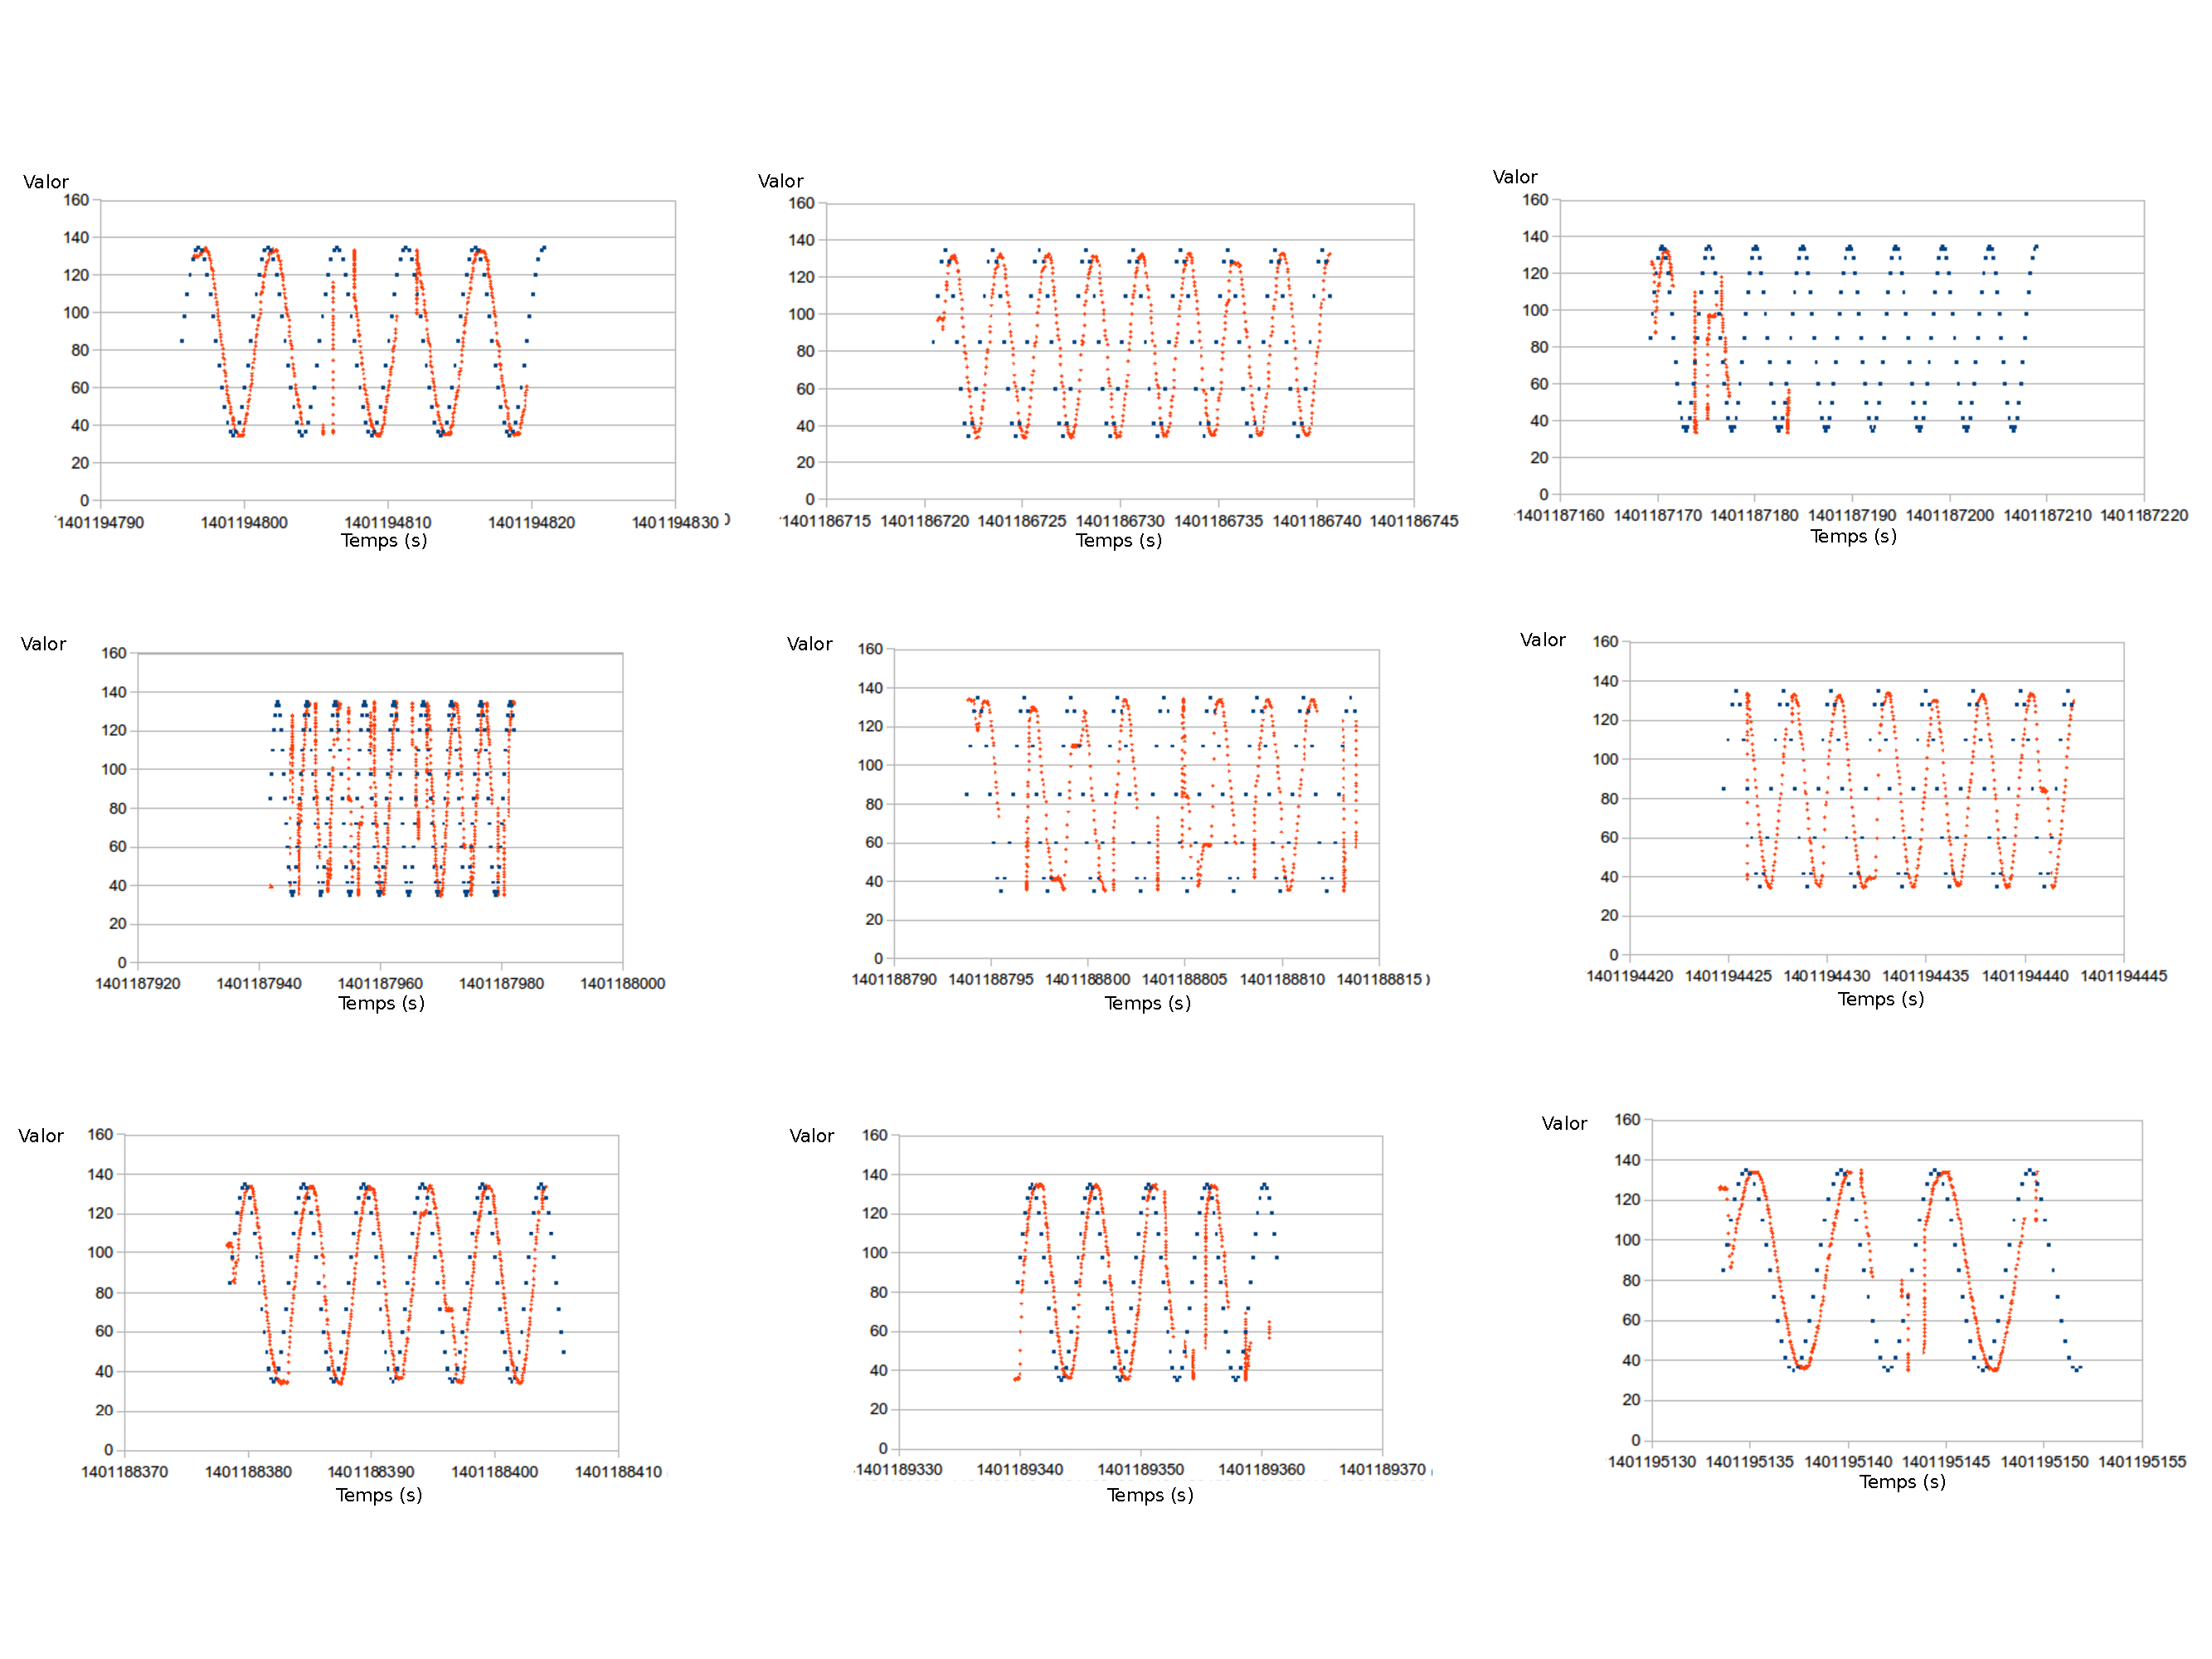
\includegraphics[scale=0.3]{images/sin5H.pdf}
	 \caption{En blau està graficat les posicions enviades a una freqüència d'5Hz i en vermell les lectures realitzades. En columnes es troben les repliques del mateix experiment i per files els tres mètodes usats, començant per liburbi amb un client, liburbi amb dos clients i telnet.}
  \label{fig:sin5H}
\end{figure}
\begin{figure}[H]
	\centering
    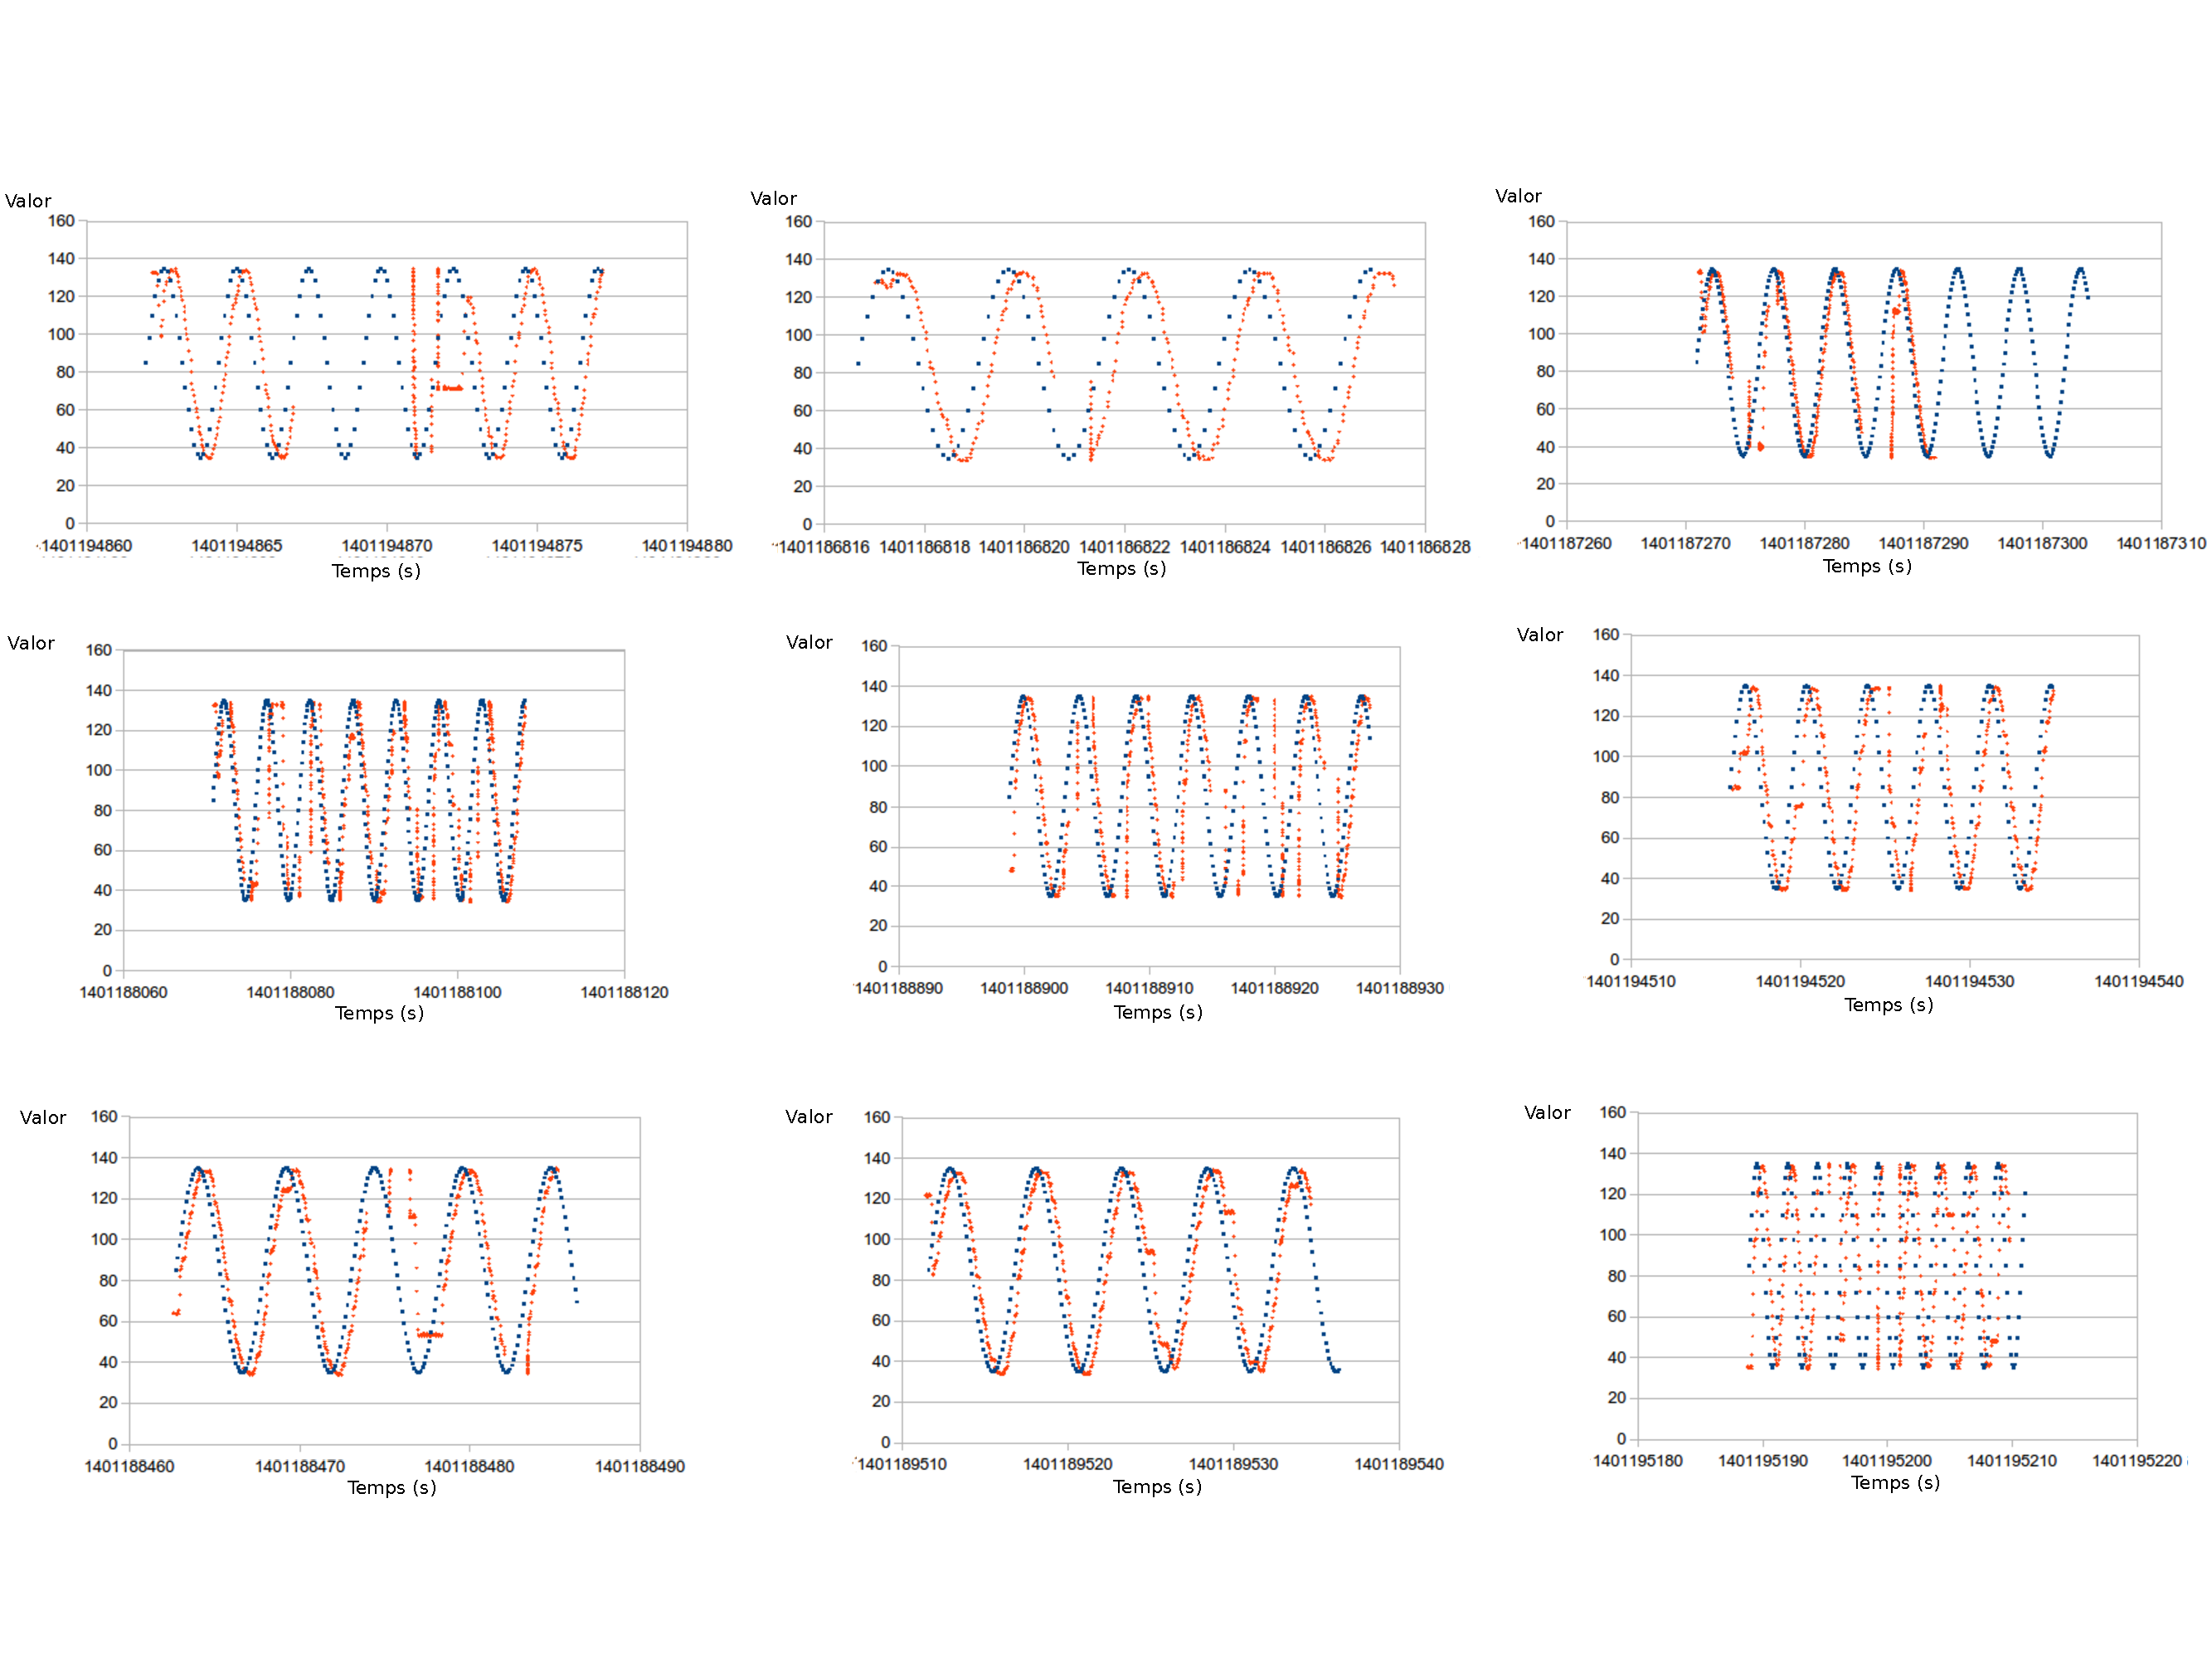
\includegraphics[scale=0.3]{images/sin10H.pdf}
	 \caption{En blau està graficat les posicions enviades a una freqüència d'10Hz i en vermell les lectures realitzades. En columnes es troben les repliques del mateix experiment i per files els tres mètodes usats, començant per liburbi amb un client, liburbi amb dos clients i telnet.}
  \label{fig:sin10H}
\end{figure}
En aquest experiment es poden trobar dos tipus d'errors que no permeten el seguiment d'una trajectoria:
\begin{itemize}
\item L'articulació no es mou: Això queda reflexat com una recta horitzontal durant un cert temps dels valors recollits en els gràfics anteriors.
\item No es rep la posició: Queda reflexat amb un període sense dades de recepció. En aquest cas no es pot saber si l'articulació es movia o no\footnote{Per inspecció visual s'ha pogut comprovar que els dos errors eren ocmpletament independents.}
\end{itemize}
El cas en que s'utilitza liburbi amb un sol client te grans buits en la recepció de dades i es el sistema en que l'articulació es mou pitjor. Pel que fa als altres programes No es pot concluir quin metode es milló amb les figures \ref{fig:sin1H} \ref{fig:sin2H} \ref{fig:sin5H} \ref{fig:sin10H}, però s'ha mirat el temps de resposta com un altre criteri d'avaluació.
 
S'agafen les diferencies dels temps en que s'envia l'ordre dels pics de la sinusoide fins al moment en que l'articulació hi arriba. La comparació es fa sobre la freqüència de 10 Hz. Realitzant una ANOVA sobre les dades obtingudes es pot dir que amb un interval de confiança del 0.95 es pot dir que el temps de retras del programa en C++ és major.
\begin{table}[H]
\begin{center}
\begin{tabulary}{\textwidth}{|p{4cm}|p{3cm}|p{3cm}|p{3cm}|}
\hline
\textbf{Python} & \textbf{C++}  \\ \hline
0.2645001411438 &	0.89370012283325  \\ \hline
0.53448987007141&	1.97295999526978 \\ \hline
1.00108003616333&	0.57231998443604 \\ \hline
0.53938007354736&	0.86796998977661 \\ \hline
0.56873989105225&	1.23644995689392 \\ \hline
0.36583995819092&	0.88230991363525 \\ \hline
0.43079996109009&	1.08385014533997 \\ \hline
0.49660015106201&	0.34201002120972 \\ \hline
0.44481992721558&	1.24258995056152 \\ \hline
0.67379021644592&	0.53582000732422 \\ \hline
0.4376699924469	&0.32669997215271 \\ \hline
0.38997006416321&	0.35342001914978 \\ \hline
1.02151989936829&	0.28936004638672 \\ \hline
0.39364004135132&	0.61238980293274 \\ \hline
0.4789400100708&	0.56062984466553 \\ \hline
0.33033013343811&	0.46492981910706 \\ \hline
0.38224005699158&	0.58044004440308 \\ \hline
0.50603008270264&	0.8042299747467 \\ \hline
0.45465016365051&	0.37677979469299  \\ \hline

\end{tabulary}
\end{center}
\caption{Retrà.\label{delay}}
\end{table}

\subsection{Elecció del mètode}
Amb els resulats anteriors es pot escollir ja el mètode més adequat per establir la comunicació am l'AIBO i es pot garantir que el seu correcte funcionament. La Taula \ref{comp} es troben resumits els resultats dels experiments realitzats.

\begin{table}[H]
\begin{center}
\begin{tabulary}{\textwidth}{|p{4cm}|p{3cm}|p{3cm}|p{3cm}|}
\hline

&\textbf{Python amb Telnet} & \textbf{C++ amb liburbi i 1 client} & \textbf{C++ amb liburbi i 2 clients} \\ \hline
Freqüencial màxima de lectura & - & + & + \\ \hline
Freqüencial mitjana de lectura & - & + & +  \\ \hline
Congelacions de les dades & = & = &= \\ \hline
Freqüencial de enviament de dades & = & = & = \\ \hline
Seguiment de trajectòries & + & - & + \\ \hline
Efecte negatiu de l'enviament sobre la lectura& - & + & - \\ \hline
Retràs de la resposta & - & + & \\ \hline
\end{tabulary}
\end{center}
\caption{Comparació dels mètodes usats i els seus resultats en els experiments.\label{comp}}
\end{table}
Els millors resultats es donen amb liburbi i dos clients a excepció del temps de resposta, que el script de python dona uns temps millors
\subsection{Possibles millores}
\section{Implementació del paquet de ROS}
\subsection{ROS}
\label{ros}
ROS és un marc de treball que proporciona eines i llibreries per ajudar als desenvolupadors de software a crear aplicacions per a robots. Proporciona entre altres abstraccions de hardware,controladors per a dispositius, eines de visualització, comunicació per missatges, administració de paquets i tot es troba sota llicencia de software lliure.

La principal característica sobre la que es basa ROS és la comunicació que proporciona. A baix nivell esta basada en pas de missatges els quals poden ser llegits o enviats per diversos processos. Aquests missatges s'escriuen sobre uns canals de comunicació anomenats \textit{tòpics} als que s'hi pot accedir mitjançant els mètodes de publicació/subscripció. La comunicació es realitza entre objectes anomenats nodes que poden subscriure's i publicar en els diferents tòpics. Tots els nodes sobre els que es vol fer comunicacions s'han de crear sobre el mateix nucli. 

\subsection{Paquet AiboServer }
L'objectiu que es persegueix amb aquest paques és un paquet que al llençar-se es conecti al AIBO que se li indiqui per direcció IP i crei un node de ROS el cual publiqui sobre uns tòpics els valors de les articulacions i sensors i estigui subscrit a un tòpic on esperi les publicacions per enviar les ordres a l'AIBO.

\begin{figure}[H]
	\centering
    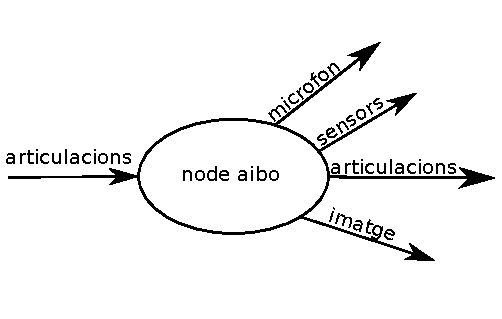
\includegraphics[scale=1]{images/aiboserver.pdf}
	 \caption{Esquema de l'objectiu buscat per a l'aibo server.}
  \label{fig:aiboserv}
\end{figure}


\subsection{Paquet AiboMimic}
\section{Cooperació i Sincronització}
\section*{Conclusions}
\addcontentsline{toc}{section}{Conclusions}




\newpage
\clearpage
\addcontentsline{toc}{section}{Referències}
\begin{thebibliography}{99}
\bibitem{kuka}
	\emph{KUKA Robotics},
	\url{http://www.kuka-robotics.com}
\bibitem{telnet}
	\emph{Telnet},
	\url{http://www.telnet.org/}
\bibitem{nasa}
	\emph{National Aeronautics and Space Administration},
	NASA.
	\url{http://www.nasa.gov/}
\bibitem{darpa}
	\emph{Defense Advanced Research Projects Agency},
	DARPA.
	\url{http://www.darpa.mil}
\bibitem{bosdin}
	\emph{Boston Dinamics},
	\url{http://www.bostondynamics.com/}
\bibitem{asimo}
	\emph{ASIMO}, 
	The world most advanced Humanoid Robot.
	HONDA
	\url{http://asimo.honda.com/}
\bibitem{wifibot}
	\emph{Wifibot}, 
	
	\url{http://www.wifibot.com/}
\bibitem{lego}
	\emph{Lego Mindstorm NXT}, 
	
	\url{http://www.lego.com/en-us/mindstorms/?domainredir=mindstorms.lego.com}
\bibitem{nao}
	\emph{Adebaran Robotics},
	NAO
	\url{http://www.aldebaran.com/en}

\bibitem{libroblanco}
	CEA, Comité Español de Automàtica,
	\emph{El libro blanco de la robòtica en España}.
	2011.
\bibitem{OPEN-R PG}
  Sony Corporation,
  \emph{OPEN-R Programmer's Guide}.
  2004.
\bibitem{xavi}
	Xavier Perez,
	\emph{Vision-based Navigation and Reinforcement Learning Path Finding for Social Robots}.
	2010.
\bibitem{metod}
	Ángel Montero Mora, Gustavo Méndez Muñoz, José Ramon Dominguez Rodriguez,
	\emph{Metodologías de diseño de comportamientos para AIBO ERS7}.
	2009.
\bibitem{robocup}
	RoboCup, \url{http://www.robocup2014.org/}
\bibitem{morales}
	Jesus Morales,
	\emph{Localización de objetos y posicionamiento en el escenario de RoboCup Four-Legged con un robot AIBO}.
	2007.  
\bibitem{jesus}
	Jesús Martinez Gómez, 
	\emph{Diseño de un teleoperador con detección de colisiones para robots AIBO}. 			2006.
\bibitem{riki}
	Ricardo A. Tellez,
	\emph{Aibo Programming}.
	\url{http://www.ouroboros.org/aibo.html}
\bibitem{TekkQuickRef}
	Ethan Tira-Thompson,
	\emph{Tekkotsu Quick Reference}, ERS-7, Tekkotsu 3.0.
\bibitem{tekkTut}
	David S. Touretzky and Ethan J. Tira-Thompson, 
	\emph{Exploring Tekkotsu Programming on Mobile Robots}.
	Carnegie Mellon University,
	2010.
	\url{http://www.cs.cmu.edu/~dst/Tekkotsu/Tutorial/contents.shtml}
\bibitem{urbi}
	\emph{URBI},
	\url{http://www.urbiforge.org/index.php/Main/Robots}
\bibitem{urbicmd}
	Jean-Christophe Baillie,
	\emph{URBI Doc for Aibo ERS2xx ERS7 Devices documentation}.
	2005.
	
\end{thebibliography}

\label{Referencies}
%\addcontentsline{toc}{section}{Referències}
%\bibliography{Aibobib.bib}

\appendix
\clearpage % o \cleardoublepage
\addappheadtotoc
\appendixpage
\section{Configuració dels marcs de treball }

\subsection{URBI}
\subsection{Tekkotsu}
\subsection{OPEN-R SDK}
\subsection{Configuració wifi}

\section{URBI}
\label{urbiA}
\section{Scripts i programes}
\subsection{Obtenció dels valors d'una variable usant liburbi per C++}
\label{getDataOneLegC++}
\lstinputlisting[language=c++]{src/getDataOneLeg/getDataC++/getData.cpp}
\subsection{Obtenció dels valors d'una variable usant una conexió telnet i python}
\label{getDataOneLegPy}
\lstinputlisting[language=Python]{src/getDataOneLeg/getDataPython/getData.py}
\subsection{Obtenció dels valors de totes les articulacions usant liburbi per C++}

\subsection{Obtenció dels valors de totes les articulacions usant una conexió telnet i python}
\subsection{Moviment d'una articulació de forma sinusoïdal usant liburbi per C++}\label{sinC}
\subsection{Moviment d'una articulació de forma sinusoïdal usant una conecció telnet i python}\label{sinP}
\end{document}
